% ============================================================================
%  The Weight of the Adjoint  -- TMLR submission
% ============================================================================
\documentclass[11pt]{article}

\usepackage[letterpaper,margin=1in]{geometry}
\usepackage{amsmath,amssymb,amsthm}
\usepackage{mathtools}
\usepackage{graphicx}
\usepackage{booktabs}
\usepackage{multirow}
\usepackage{array}
\usepackage{xcolor}
\usepackage{microtype}
\usepackage[round,authoryear]{natbib}
\usepackage[colorlinks=true,linkcolor=blue!55!black,citecolor=blue!55!black,urlcolor=blue!55!black]{hyperref}
\usepackage{caption}
\usepackage{tikz}
\usetikzlibrary{positioning,arrows.meta,fit,backgrounds,calc,shapes.geometric}
\captionsetup{font=small,labelfont=bf}

% --- float placement ---------------------------------------------------------
% This document is float-dense. With the stock parameters LaTeX's deferral queue
% backs up and dumps the results figures after the bibliography, where they read
% as an appendix. Relax the limits and forbid floats from crossing a section.
\usepackage[section]{placeins}
\setcounter{topnumber}{3}
\setcounter{bottomnumber}{2}
\setcounter{totalnumber}{4}
\renewcommand{\topfraction}{0.9}
\renewcommand{\bottomfraction}{0.7}
\renewcommand{\textfraction}{0.08}
\renewcommand{\floatpagefraction}{0.75}

\newtheorem{theorem}{Theorem}
\newtheorem{proposition}[theorem]{Proposition}
\newtheorem{lemma}[theorem]{Lemma}
\theoremstyle{definition}
\newtheorem{definition}[theorem]{Definition}
\theoremstyle{remark}
\newtheorem{remark}[theorem]{Remark}

\newcommand{\R}{\mathbb{R}}
\newcommand{\iprod}[2]{\langle #1, #2 \rangle}
\newcommand{\defect}{\mathcal{D}}
\newcommand{\Wc}{W_{\mathrm{cheb}}}
\newcommand{\Wu}{W_{\mathrm{unif}}}
\newcommand{\sacheb}{\textsc{SA-Cheb}}
\newcommand{\ckino}{\textsc{CKINO}}

% --- palette shared with the figures -----------------------------------------
\definecolor{cCheb}{HTML}{C1272D}
\definecolor{cUnif}{HTML}{0B6E4F}
\definecolor{cBox}{HTML}{FFF3C4}
\definecolor{cOrange}{HTML}{E8A33D}
\definecolor{cBlue}{HTML}{7FB3D5}
\definecolor{cRed}{HTML}{E05C4A}
\definecolor{cGrey}{HTML}{6C757D}

\title{\bfseries\LARGE The Weight of the Adjoint\\[6pt]
\large Which Symplectic Form a Neural Operator Preserves,\\
and Whether It Survives the Lift}

\author{
  \textbf{Sourav Sahu} \\ Microsoft \\ \texttt{sahusourav@microsoft.com}
  \and
  \textbf{Gareth O'Brien} \\ Microsoft \\ \texttt{O.Gareth@microsoft.com}
}
\date{}

\begin{document}
\maketitle

\begin{abstract}
Structure-preserving neural operators are built on a question that is usually
left unasked: symplectic \emph{with respect to which inner product}? On a
non-uniform grid the discrete $L^2$ adjoint is $K^{*}=W^{-1}K^{\top}W$, where
$W$ collects the quadrature weights, and the choice of $W$ silently selects
which symplectic form a gradient shear preserves. We make that choice explicit,
build both alternatives, and measure them. Using the symplectic defect
$\lVert WA-A^{\top}W\rVert_F/\lVert WA\rVert_F$ computed from the autograd
Jacobian, we find a clean diagonal across $1$-D, $2$-D and $3$-D: each
construction is exact ($2\times10^{-16}$) in the form its adjoint was built from
and $O(1)$ away from the other. Preserving \emph{a} symplectic form is therefore
cheap; the content lies entirely in preserving the \emph{right} one. Because our
benchmarks are discretised on uniform grids, this yields a controlled test, and
the matched-form operator wins $16$ of $18$ paired comparisons. When we remove
the lift and projection layers so that the \emph{deployed map}, rather than merely its interior blocks, is symplectic, the margin widens to $14$--$22\times$. The same
construction then produces the study's strongest result: over a $2\times10^{4}$
step rollout every operator we tested diverges to relative errors of
$10^{5}$--$10^{12}$, \emph{except} the lift-free symplectic ones, which remain
bounded at relative error of order unity. That is stability rather than
accuracy, but it separates them from everything else by five to twelve orders of
magnitude. Structure preservation is not
a cost, as a prior version of this study concluded; it is a benefit that is
forfeited by the conventional lift--process--project wrapper and invisible
unless the inner product is named. We also report a $783$-run, nine-equation,
three-seed benchmark, and retract an earlier symplecticity theorem of our own
that conflated unit Jacobian determinant with preservation of $\omega$.
\end{abstract}

% ============================================================================
\section{Introduction}
% ============================================================================

Neural operators learn maps between function spaces and are now widely studied
as surrogates for parametric PDEs \citep{kovachki2023neural,li2021fno,lu2021deeponet}.
A fast-growing branch argues that such operators should respect the
\emph{geometric structure} of the dynamics they emulate: symplecticity for Hamiltonian systems, or the metriplectic split when dissipation is present. The
argument has a strong pedigree in finite dimensions
\citep{greydanus2019hnn,jin2020sympnets,cranmer2020lnn,zhong2020symoden}, and in
2026 several groups carried it into function space
\citep{makara2026sno,sulskis2026generic,zhang2026legonet,varghese2026pisonet}.

Two things are left implicit across the work we reviewed. First, whether a
trained network is actually structure-preserving is argued on paper rather than
measured. Second, and this is our starting point, the claim is stated without
naming the inner product it is relative to. On a uniform grid that omission is
harmless, because the quadrature weight is a single scalar. On a non-uniform
grid it is not: the weights vary by a factor of order $N$
(Figure~\ref{fig:weights}), the adjoint is $K^{*}=W^{-1}K^{\top}W$ rather than
$K^{\top}$, and two implementations that differ only in which $W$ they assume
preserve two \emph{different} symplectic forms.

This gives an unusually clean experiment. Build both, verify that each is exact
in its own form, then ask which one helps. Our contributions:

\label{sec:intro-claims}
\begin{enumerate}\itemsep2pt
\item \textbf{An instrument} (\S\ref{sec:defect}). We measure the symplectic
defect directly from the autograd Jacobian, against \emph{both} candidate inner
products, scaling to $3$-D with Hutchinson probes. It first falsified a
symplecticity claim in our own earlier work (Appendix~\ref{app:retraction}).

\item \textbf{A construction} (\S\ref{sec:arch}). \sacheb{}: exact symplecticity
on a non-periodic Chebyshev grid in $1$-D, $2$-D and $3$-D, for any kernel and
any pointwise nonlinearity (Theorem~\ref{thm:sacheb}). We describe it and the
\ckino{} operator it grew out of component by component.

\item \textbf{The form result} (\S\ref{sec:form}). Each variant is exact in its
own form and $O(1)$ in the other. The variant whose form matches the grid wins
$16/18$ paired comparisons; with the lift removed, $4/4$ by $14$--$22\times$.

\item \textbf{The lift result} (\S\ref{sec:long}). Only operators that are
symplectic \emph{end to end} survive a $2\times10^{4}$-step rollout. A symplectic
core wrapped in pointwise lift, projection and a residual update does not.

\item \textbf{A benchmark} (\S\ref{sec:setup}): $783$ runs over nine equations in
$1$-D/$2$-D/$3$-D at matched capacity, three seeds, plus an
unconstrained-capacity sweep showing the ranking is budget-dependent.
\end{enumerate}

\paragraph{A correction.} An earlier version of this study reported that exact
symplecticity was a measurable \emph{cost}. That conclusion was an artefact of
scoring both variants against a single inner product. We state the error plainly
here because it is the kind the instrument exists to catch.

% ============================================================================
\section{Related work}
% ============================================================================

\paragraph{Neural operators.} The Fourier Neural Operator parameterises the
integral kernel by truncated Fourier multipliers \citep{li2021fno}, inheriting
discretisation invariance and $O(N\log N)$ cost; DeepONet factorises the operator
into branch and trunk networks \citep{lu2021deeponet}; the general framework and
universality results are due to \citet{kovachki2023neural}. Tensorised
\citep{kossaifi2023mgtfno} and U-Net-augmented \citep{wen2022ufno} variants
improve parameter efficiency. A practitioner-oriented account of FNO's
assumptions is given by \citet{duruisseaux2026fnoexplained}, with reference
implementations in \citet{kossaifi2024library}. Physics-informed variants add PDE
residuals to the loss \citep{raissi2019pinn,li2023pino}; these are \emph{soft}
constraints with no algebraic guarantee.

\paragraph{Structure preservation in finite dimensions.} Hamiltonian
\citep{greydanus2019hnn} and Lagrangian \citep{cranmer2020lnn} neural networks
learn the generating function; SympNets \citep{jin2020sympnets} and Symplectic
ODE-Net \citep{zhong2020symoden} parameterise symplectic maps directly. These act
on $\R^{2d}$ at a fixed discretisation and are not operators in the
function-space sense.

\paragraph{Structure-preserving neural operators.} \citet{makara2026sno}
introduce the Symplectic Neural Operator (SNO), composing symplectic shear blocks
whose update fields are gradients of learned energy functionals, realised with
self-adjoint Fourier layers on the torus. \citet{sulskis2026generic} embed the
GENERIC degeneracy structure \citep{grmela1997generic,ottinger2005beyond} into an
FNO, extending finite-dimensional bracket learning \citep{zhang2022gfinns}.
\citet{zhang2026legonet} compose structure-preserving blocks on boundary-adapted
spectral representations, and \citet{varghese2026pisonet} apply a conditional
symplectic operator to optimal control.

\paragraph{Where we differ.} All of these are built on the torus or on a uniform
grid, where $W\propto I$ and the adjoint question does not arise, so the correct adjoint is obtained \emph{by accident}. \citet{makara2026sno} state explicitly
that their formulation covers strong canonical symplectic Hilbert spaces and that
extensions require further machinery. We work in the setting where the choice is
forced, show that it is consequential, and measure rather than assert the
outcome. Auxiliary ingredients we use, namely Lie-equivariant lifting
\citep{finzi2020lieconv} and FiLM conditioning \citep{perez2018film}, are standard and not claimed as contributions.

% ============================================================================
\section{Background: symplectic structure on a non-uniform grid}
\label{sec:background}
% ============================================================================

\subsection{Notation}
\label{sec:notation}

Table~\ref{tab:notation} collects every symbol used in the paper. Vectors are
columns, $^{\top}$ is the plain matrix transpose, and $^{*}$ is reserved for the
adjoint with respect to a weighted inner product; the distinction between the two is the subject of the paper.

% deliberately NOT a float: the reader must meet the notation before the algebra
\begin{center}
\captionof{table}{Symbols and notation.}
\label{tab:notation}
\small
\begin{tabular}{@{}llp{78mm}@{}}
\toprule
symbol & reads as & meaning \\
\midrule
$\Omega_{\mathrm{d}}$ & & spatial domain, taken as $[-1,1]$ in $1$-D \\
$d$ & & number of spatial dimensions, $d\in\{1,2,3\}$ \\
$N$ & & grid index; a $1$-D grid carries $N{+}1$ nodes \\
$x_j=\cos(j\pi/N)$ & & Chebyshev--Gauss--Lobatto (CGL) nodes \\
$w_j>0$ & & quadrature weight at node $j$ \\
$W=\mathrm{diag}(w_j)$ & & weight matrix; \emph{diagonal and positive} \\
$\Wc$, $\Wu$ & & the two candidate weight matrices: Clenshaw--Curtis weights on CGL nodes, and constant weights (a uniform grid) \\
$\iprod{f}{g}_W=f^{\top}Wg$ & ``$f$ dot $g$ in $W$'' & discrete $L^2$ inner product \\
$K$ & & a linear (kernel-integral) operator \\
$K^{\top}$ & ``$K$ transpose'' & matrix transpose \\
$K^{*}=W^{-1}K^{\top}W$ & ``$K$ adjoint'' & adjoint \emph{with respect to} $\iprod{\cdot}{\cdot}_W$ \\
$q,p$ & & the two halves of a canonical phase-space state \\
$z=(q,p)$ & & a point of phase space $\mathbb{P}$ \\
$\omega_W$ & ``omega'' & symplectic form induced by $W$, eq.~\eqref{eq:omega} \\
$\Omega$ & & matrix of $\omega_W$, eq.~\eqref{eq:omega} \\
$\Phi$ & ``Phi'' & one shear map of phase space \\
$D\Phi$ & & Jacobian of $\Phi$ \\
$F,G$ & & the update (shear) fields \\
$A=DF$ & & Jacobian of the shear field \\
$R$, $\rho=R'$ & ``rho'' & scalar potential and its derivative, applied pointwise \\
$D=\mathrm{diag}(\rho'(\cdot))$ & & diagonal matrix of pointwise slopes \\
$\mathcal{E}$ & ``script E'' & learned energy functional \\
$\nabla_W$ & ``grad in $W$'' & gradient with respect to $\iprod{\cdot}{\cdot}_W$ \\
$\varphi_r,\psi_r$ & ``phi, psi'' & the $r$-th left/right basis functions of the kernel \\
$M_r$ & & channel-mixing matrix of mode $r$ \\
$R$ (rank) & & Mercer rank; context distinguishes it from the potential $R$ \\
$\sigma_r$ & ``sigma'' & learned positive Mercer scale \\
$C$, $H$ & & physical and hidden channel counts \\
$\defect_W$ & ``defect'' & relative symplectic defect, eq.~\eqref{eq:defect} \\
$\lVert\cdot\rVert_F$ & ``Frobenius norm'' & $\lVert X\rVert_F^2=\sum_{ij}X_{ij}^2$ \\
$[S,M]=SM-MS$ & ``commutator'' & used in Proposition~\ref{prop:necessity} \\
\bottomrule
\end{tabular}
\end{center}

\subsection{The discrete inner product}

Let $\Omega_{\mathrm{d}}=[-1,1]$ be discretised on the $N+1$ CGL nodes
$x_j=\cos(j\pi/N)$. Functions are represented by nodal values, and the physical
$L^2$ product is approximated by Clenshaw--Curtis quadrature
\citep{trefethen2000spectral},
\begin{equation}
\iprod{f}{g}_W \;=\; \int_{\Omega_{\mathrm{d}}} f g\,dx \;\approx\; f^{\top} W g,
\qquad W=\mathrm{diag}(w_0,\dots,w_N),\quad w_j>0 .
\label{eq:ip}
\end{equation}

\begin{figure}[htbp]
\centering
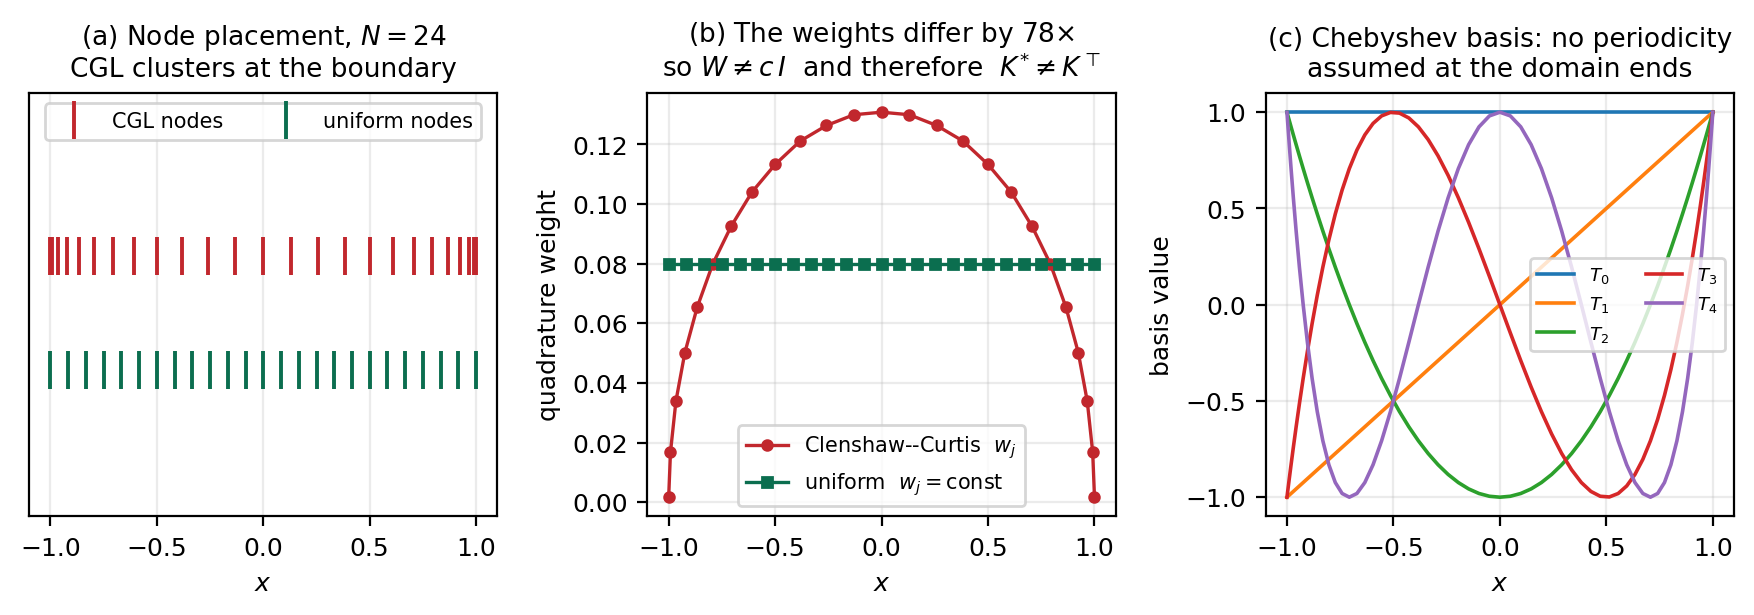
\includegraphics[width=\linewidth]{figs/weights.png}
\caption{The geometric fact the paper rests on. \textbf{(a)} CGL nodes cluster
quadratically at the boundary; a uniform grid does not. \textbf{(b)} The
Clenshaw--Curtis weights therefore vary by $78\times$ across the domain at
$N=24$, so $W\neq cI$ and consequently $K^{*}\neq K^{\top}$. On a uniform grid
the two coincide, which is why a Fourier-parameterised operator using the
standard uniform quadrature does not meet the distinction. \textbf{(c)} The
Chebyshev basis assumes no periodicity at the domain ends.}
\label{fig:weights}
\end{figure}

Phase space is $\mathbb{P}=\mathcal{H}_q\oplus\mathcal{H}_p$ with
$\mathcal{H}=(\R^{N+1},\iprod{\cdot}{\cdot}_W)$, carrying
\begin{equation}
\omega_W(z,z') = \iprod{q}{p'}_W - \iprod{p}{q'}_W = z^{\top}\Omega z',
\qquad
\Omega=\begin{pmatrix} 0 & W \\ -W & 0\end{pmatrix}.
\label{eq:omega}
\end{equation}
This is the finite-dimensional shadow of the weak symplectic form on a Hilbert
phase space \citep{weinstein1969symplectic,marsden1999mechanics}; the point of
what follows is that the discretisation chooses $W$, and that choice is not
innocuous.

\begin{definition}[Weighted adjoint]
The adjoint of $K$ with respect to \eqref{eq:ip} is the unique $K^{*}$ with
$\iprod{Kf}{g}_W=\iprod{f}{K^{*}g}_W$ for all $f,g$. Expanding,
$f^{\top}K^{\top}Wg=f^{\top}WK^{*}g$, hence
\begin{equation}
\boxed{\;K^{*}=W^{-1}K^{\top}W\;}
\label{eq:adjoint}
\end{equation}
\end{definition}

\begin{proposition}[Shear criterion]
\label{prop:shear}
Let $\Phi(q,p)=(q,\,p+F(q))$ with $A=DF(q)$. Then
\begin{equation}
(D\Phi)^{\top}\Omega\,(D\Phi)-\Omega
=\begin{pmatrix} WA - A^{\top}W & 0\\ 0 & 0\end{pmatrix},
\label{eq:defect-identity}
\end{equation}
so $\Phi$ preserves $\omega_W$ \emph{iff} $A$ is self-adjoint in $W$, i.e.\
$WA=A^{\top}W$. The transposed shear behaves analogously.
\end{proposition}

\begin{proof}
$D\Phi=\begin{psmallmatrix} I&0\\ A&I\end{psmallmatrix}$, so
$\Omega D\Phi=\begin{psmallmatrix} WA& W\\ -W&0\end{psmallmatrix}$ and
$(D\Phi)^{\top}\Omega D\Phi
=\begin{psmallmatrix} I&A^{\top}\\ 0&I\end{psmallmatrix}
 \begin{psmallmatrix} WA& W\\ -W&0\end{psmallmatrix}
=\begin{psmallmatrix} WA-A^{\top}W& W\\ -W&0\end{psmallmatrix}$.
Subtract $\Omega$.
\end{proof}

\begin{remark}[Volume preservation is not symplecticity]
\label{rem:volume}
$\det D\Phi=1$ for \emph{every} shear, whatever $A$. Unit Jacobian determinant is
Liouville volume preservation, strictly weaker than preservation of $\omega_W$,
which by Proposition~\ref{prop:shear} additionally requires $WA=A^{\top}W$.
Conflating the two is, in our experience, the most common way an architecture
described as symplectic turns out not to be; we exhibit an instance of our own in
\S\ref{sec:form} and Appendix~\ref{app:retraction}.
\end{remark}

\begin{remark}[The question is under-specified]
\label{rem:illposed}
Because \eqref{eq:defect-identity} depends on $W$, ``is this block symplectic?''
has no answer until $W$ is named. Two implementations differing only in the $W$
used inside the adjoint are \emph{both} exactly symplectic, in different forms.
This is the observation the rest of the paper develops.
\end{remark}

% ============================================================================
\section{Architectures}
\label{sec:arch}
% ============================================================================

We describe two operators. \ckino{} is a Chebyshev kernel-integral operator that
motivated this study and serves as our non-periodic baseline; \sacheb{} is the
self-adjoint construction that makes the symplectic form explicit and
controllable.

\subsection{\ckino{}: a Chebyshev kernel-integral operator}
\label{sec:ckino}

\ckino{} replaces FNO's Fourier multipliers with a low-rank kernel expanded in
\emph{Chebyshev coefficients}, so that no periodicity is assumed and the operator
can be evaluated on any CGL grid. Figure~\ref{fig:ckino} shows the pipeline; the
components are as follows.

\begin{figure}[htbp]
\centering
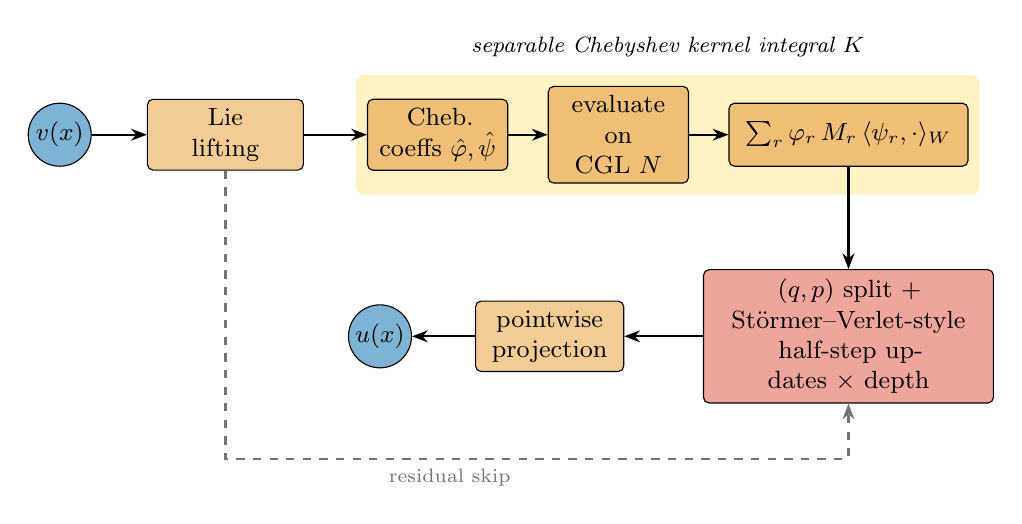
\begin{tikzpicture}[
  font=\small,
  node distance=6mm,
  box/.style={draw,rounded corners=2pt,minimum height=8mm,inner xsep=4pt,align=center},
  circ/.style={draw,circle,minimum size=8mm,inner sep=1pt},
  ar/.style={-{Stealth[length=2mm]},thick}
]
\node[circ,fill=cBlue] (in) {$v(x)$};
\node[box,fill=cOrange!55,right=7mm of in,text width=17mm] (lift)
     {Lie\\lifting};
% --- kernel integral group ---
\node[box,fill=cOrange!70,right=8mm of lift,text width=15mm] (coef)
     {Cheb.\\coeffs $\hat\varphi,\hat\psi$};
\node[box,fill=cOrange!70,right=5mm of coef,text width=15mm] (eval)
     {evaluate\\on CGL $N$};
% no text width: let the node grow to fit the formula, otherwise it spills
% out of the shaded group box behind it
\node[box,fill=cOrange!70,right=5mm of eval,inner xsep=6pt] (contract)
     {$\sum_r \varphi_r\, M_r\, \langle \psi_r, \cdot\rangle_W$};
\begin{scope}[on background layer]
  \node[fill=cBox,rounded corners=3pt,fit=(coef)(eval)(contract),inner sep=4pt] (kbox) {};
\end{scope}
\node[above=1mm of kbox,font=\footnotesize\itshape] {separable Chebyshev kernel integral $K$};
% --- symplectic-style block ---
\node[box,fill=cRed!55,below=13mm of contract,text width=34mm] (blk)
     {$(q,p)$ split $+$ St\"ormer--Verlet-style\\ half-step updates $\times$ depth};
\node[box,fill=cOrange!55,left=10mm of blk,text width=16mm] (proj) {pointwise\\projection};
\node[circ,fill=cBlue,left=8mm of proj] (out) {$u(x)$};

\draw[ar] (in) -- (lift);
\draw[ar] (lift) -- (coef);
\draw[ar] (coef) -- (eval);
\draw[ar] (eval) -- (contract);
\draw[ar] (contract) -- (blk);
\draw[ar] (blk) -- (proj);
\draw[ar] (proj) -- (out);
\coordinate (rb) at ($(blk.south)+(0,-7mm)$);
\draw[ar,cGrey,dashed] (lift.south) |- (rb)
      node[pos=0.68,below,font=\scriptsize,text=cGrey] {residual skip}
      -- (blk.south);
\end{tikzpicture}
\caption{\ckino{}. The kernel is stored as Chebyshev \emph{coefficients} and
evaluated on whatever CGL grid is requested, so the parameters are independent of
resolution. The $(q,p)$ block mimics a St\"ormer--Verlet half-step. Its Jacobian
is triangular with unit diagonal, hence volume-preserving; but as \S\ref{sec:form} shows by measurement, \emph{not} symplectic in either candidate
form.}
\label{fig:ckino}
\end{figure}

\paragraph{(i) Lie-equivariant lifting.} A pointwise or short-stencil map raising
the $C$ physical fields to $H$ hidden channels, built from generators of a small
Lie group so that the lift commutes with translations of the input
\citep{finzi2020lieconv}. Two variants matter later: a \emph{convolutional} lift
(resolution-dependent stencil) and a \emph{spectral} lift (FFT-derivative, exactly
resolution-invariant). \S\ref{sec:support} shows these trade invariance against
accuracy.

\paragraph{(ii) Separable Chebyshev kernel integral.} The operator core,
\begin{equation}
(Kv)(x)=\sum_{r=1}^{R}\Big(\textstyle\prod_{a=1}^{d}\varphi^a_r(x_a)\Big)\,
        \sigma_r M_r \iprod{\textstyle\prod_a\psi^a_r}{v}_W ,
\label{eq:ckino-kernel}
\end{equation}
with $\varphi^a_r,\psi^a_r$ stored as $n_{\mathrm{train}}{+}1$ Chebyshev
coefficients per axis, $M_r\in\R^{H\times H}$ mixing channels and $\sigma_r>0$ a
learned Mercer scale. Cost is $O(RN^d)$ rather than $O(N^{2d})$, and because the
basis functions are polynomials the same weights evaluate on any grid.

\paragraph{(iii) St\"ormer--Verlet-style block.} Hidden channels are split into
$(q,p)$ halves and updated by alternating half-steps with a learned step size.
This is where the original symplecticity claim was made, and where it fails:
\eqref{eq:ckino-kernel} uses \emph{independent} $\varphi_r$ and $\psi_r$ and an
unconstrained $M_r$, so nothing forces $k(x,y)=k(y,x)^{\top}$ and the Jacobian is
not self-adjoint in any of the forms we consider.

\paragraph{(iv) Projection.} A pointwise map back to $C$ output channels.

\subsection{\sacheb{}: making the form explicit}
\label{sec:sacheb}

\sacheb{} repairs (iii) by construction. Let $K$ be a bounded linear operator,
$R\in C^2(\R)$ with $\rho=R'$, and define the energy functional and its
$W$-gradient
\begin{equation}
\mathcal{E}(q)=\int_\Omega R\big((Kq)(x)\big)\,dx,
\qquad
F(q) \;=\; \nabla_W\mathcal{E}(q) \;=\; K^{*}\rho(Kq),
\label{eq:field}
\end{equation}
with $K^{*}$ the weighted adjoint \eqref{eq:adjoint}. The block alternates
\begin{equation}
\Phi^{\uparrow}(q,p)=(q,\;p+F_\theta(q)),
\qquad
\Phi^{\downarrow}(q,p)=(q+G_\vartheta(p),\;p).
\label{eq:block}
\end{equation}

\begin{figure}[htbp]
\centering
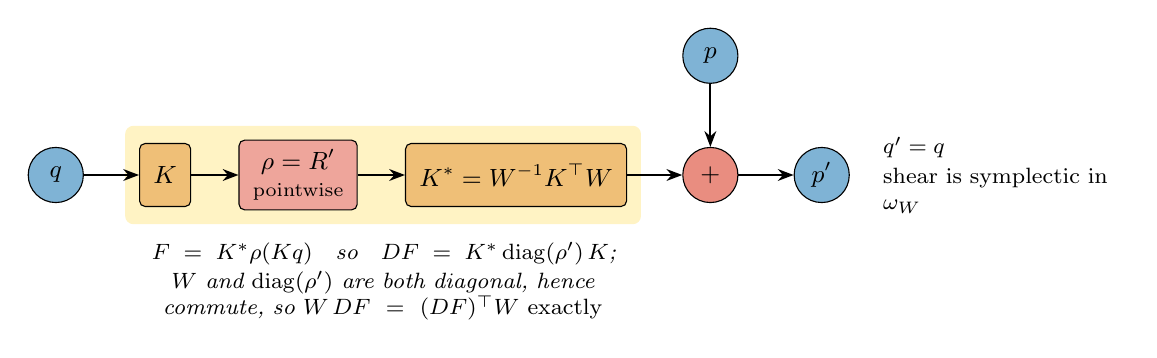
\begin{tikzpicture}[
  font=\small,
  box/.style={draw,rounded corners=2pt,minimum height=8mm,inner xsep=5pt,align=center},
  circ/.style={draw,circle,minimum size=7mm,inner sep=1pt},
  ar/.style={-{Stealth[length=2mm]},thick}
]
\node[circ,fill=cBlue] (q) {$q$};
\node[box,fill=cOrange!70,right=7mm of q] (K) {$K$};
\node[box,fill=cRed!55,right=6mm of K] (rho) {$\rho=R'$\\[-1pt]\scriptsize pointwise};
\node[box,fill=cOrange!70,right=6mm of rho] (Ks) {$K^{*}=W^{-1}K^{\top}W$};
\node[circ,fill=cRed!70,right=7mm of Ks] (plus) {$+$};
\node[circ,fill=cBlue,right=7mm of plus] (pout) {$p'$};
\node[circ,fill=cBlue,above=8mm of plus] (p) {$p$};
\draw[ar] (q) -- (K);  \draw[ar] (K) -- (rho);  \draw[ar] (rho) -- (Ks);
\draw[ar] (Ks) -- (plus); \draw[ar] (p) -- (plus); \draw[ar] (plus) -- (pout);
\begin{scope}[on background layer]
  \node[fill=cBox,rounded corners=3pt,fit=(K)(rho)(Ks),inner sep=5pt] (g) {};
\end{scope}
\node[below=1mm of g,font=\footnotesize\itshape,text width=72mm,align=center]
  {$F=K^{*}\rho(Kq)$ \; so \; $DF=K^{*}\,\mathrm{diag}(\rho')\,K$;\\[1pt]
   $W$ and $\mathrm{diag}(\rho')$ are both diagonal, hence commute,
   so $W\,DF=(DF)^{\top}W$ \emph{exactly}};
\node[right=3mm of pout,font=\footnotesize,text width=30mm,align=left]
  {$q'=q$\\[1pt] shear is symplectic in $\omega_W$};
\end{tikzpicture}
\caption{The \sacheb{} gradient shear. The only design choice is which $W$ enters
$K^{*}$: the Clenshaw--Curtis weights ($\Wc$) or constant weights ($\Wu$). Both
give an \emph{exactly} symplectic block, in different forms. That choice, not
the presence of symplecticity, is what the experiments vary.}
\label{fig:sacheb}
\end{figure}

\begin{theorem}[Exact symplecticity, any dimension]
\label{thm:sacheb}
For any parameters of $K$, any $R\in C^2$, any resolution $N$ and any spatial
dimension $d\in\{1,2,3\}$, the map $\Phi^{\uparrow}$ of \eqref{eq:block}
satisfies $(\Phi^{\uparrow})^{*}\omega_W=\omega_W$ exactly, and likewise
$\Phi^{\downarrow}$; hence so does any finite alternating composition.
\end{theorem}

\begin{proof}
Write $D=\mathrm{diag}\big(\rho'((Kq)_j)\big)$, so $A=DF=K^{*}DK$. Using
\eqref{eq:adjoint},
\[
WA = W(W^{-1}K^{\top}W)DK = K^{\top}WDK,
\qquad
A^{\top}W = K^{\top}D(K^{*})^{\top}W = K^{\top}D\,W\!KW^{-1}W = K^{\top}DWK .
\]
$W$ and $D$ are diagonal and therefore commute, so $WA=A^{\top}W$; apply
Proposition~\ref{prop:shear}. In $d$ dimensions the weight is the outer product
$W=\bigotimes_a W_a$, still diagonal, so the argument is unchanged.
\end{proof}

Theorem~\ref{thm:sacheb} says the block is symplectic in \emph{the form its
adjoint was built from}. It says nothing about any other form, and the next
result shows that the omission is not a technicality: it is the whole content of
the paper, and it predicts the pattern measured in Figure~\ref{fig:defect}.

\begin{proposition}[Which form, and only which form]
\label{prop:necessity}
Fix a positive diagonal $W_1$ and build the shear field with the adjoint taken in
$W_1$, i.e.\ $F(q)=K^{*}_{W_1}\rho(Kq)$ with $K^{*}_{W_1}=W_1^{-1}K^{\top}W_1$,
so that $A=K^{*}_{W_1}DK$. Let $W_2$ be any other positive diagonal weight. Then
\begin{equation}
W_2A - A^{\top}W_2 \;=\; [\,S,\,M\,] \;=\; SM-MS,
\qquad S := W_2W_1^{-1},\quad M := K^{\top}W_1DK ,
\label{eq:commutator}
\end{equation}
where $S$ is diagonal and $M$ is symmetric. Consequently
\begin{equation}
\big(W_2A-A^{\top}W_2\big)_{ij} = (s_i-s_j)\,M_{ij},
\label{eq:entrywise}
\end{equation}
and the shear is symplectic in $\omega_{W_2}$ \emph{for every} $K$ and $\rho$ if
and only if $W_2\propto W_1$.
\end{proposition}

\begin{proof}
Since $W_1$ is symmetric, $(K^{*}_{W_1})^{\top}=(W_1^{-1}K^{\top}W_1)^{\top}
=W_1KW_1^{-1}$. Diagonal matrices commute, so $W_1D=DW_1$ and
$W_1^{-1}W_2=W_2W_1^{-1}=S$. Then
\[
W_2A = W_2W_1^{-1}K^{\top}W_1DK = S\,\big(K^{\top}W_1DK\big) = SM ,
\]
\[
A^{\top}W_2 = K^{\top}D\,(K^{*}_{W_1})^{\top}W_2
            = K^{\top}D\,W_1KW_1^{-1}W_2
            = \big(K^{\top}W_1DK\big)S = MS ,
\]
which gives \eqref{eq:commutator}. $M$ is symmetric because
$M^{\top}=K^{\top}(W_1D)^{\top}K=K^{\top}DW_1K=K^{\top}W_1DK=M$. Writing
$S=\mathrm{diag}(s_i)$ gives $(SM-MS)_{ij}=s_iM_{ij}-M_{ij}s_j$, which is
\eqref{eq:entrywise}.

For the equivalence: if $W_2=cW_1$ then $S=cI$, every $s_i-s_j$ vanishes and so does the defect, recovering Theorem~\ref{thm:sacheb} at $c=1$. Conversely,
suppose $W_2\not\propto W_1$, so there are indices $i\neq j$ with $s_i\neq s_j$.
Choose $D=I$ (take $\rho'\equiv1$) and $K=e_ie_i^{\top}+e_je_j^{\top}$; then
$M=K^{\top}W_1K$ has $M_{ij}=0$, so pick instead
$K=(e_i+e_j)e_i^{\top}+(e_i+e_j)e_j^{\top}$, for which
$M_{ij}=(w_{1,i}+w_{1,j})\neq0$. By \eqref{eq:entrywise} the $(i,j)$ entry of the
defect is $(s_i-s_j)M_{ij}\neq0$, so the shear is not symplectic in
$\omega_{W_2}$ for that parameter choice.
\end{proof}

\begin{remark}[The defect scales with the spread of $W_2/W_1$]
\label{rem:spread}
Equation~\eqref{eq:entrywise} says the mismatch is governed entirely by the
\emph{spread} of the ratio $s_i=w_{2,i}/w_{1,i}$: a larger dynamic range in
$W_2W_1^{-1}$ produces a larger defect. This is a falsifiable prediction, and
Figure~\ref{fig:defect} bears it out: the off-diagonal entries grow from
$\approx0.7$ in $1$-D to $\approx0.95$ in $2$-D and $1.0$--$1.3$ in $3$-D,
precisely because the tensor-product weight $\bigotimes_a W_a$ has a wider
dynamic range as $d$ grows.
\end{remark}

\paragraph{Low-rank realisation.} With
$Kv=\sum_r\varphi_r M_r\iprod{\psi_r}{v}_W$ the weighted adjoint is
$K^{*}g=\sum_r\psi_r M_r^{\top}\iprod{\varphi_r}{g}_W$ (Appendix~\ref{app:lowrank}):
\emph{swap $\varphi\leftrightarrow\psi$ and transpose $M$}. No inverse of $W$ is
ever formed and the cost stays $O(RN^d)$.

\subsection{Lifted versus lift-free, and why it matters}
\label{sec:lift}

Theorem~\ref{thm:sacheb} is a statement about the \emph{block}. A deployed
operator usually wraps blocks in a pointwise lift and projection and is driven
residually, $x_{t+1}=x_t+\mathcal{N}(x_t)$. None of those three maps is
symplectic, so the composition is not either
(Figure~\ref{fig:lift}). We therefore build both:

\begin{itemize}\itemsep2pt
\item \textbf{Lifted} (\texttt{sacheb}, \texttt{sacheb\_naive}): $H\gg C$ hidden
channels, maximal capacity, symplectic \emph{core} only.
\item \textbf{Lift-free} (\texttt{sacheb\_pure}, \texttt{sacheb\_pure\_naive}):
the shears act directly on the PDE's own $(q,p)$ fields, $H=C$, no lift, no
projection, non-residual update. The \emph{deployed map} is exactly symplectic;
capacity must come from rank and depth instead. This requires a canonical
$(q,p)$ pair and so applies only to two-field problems.
\end{itemize}

\begin{figure}[htbp]
\centering
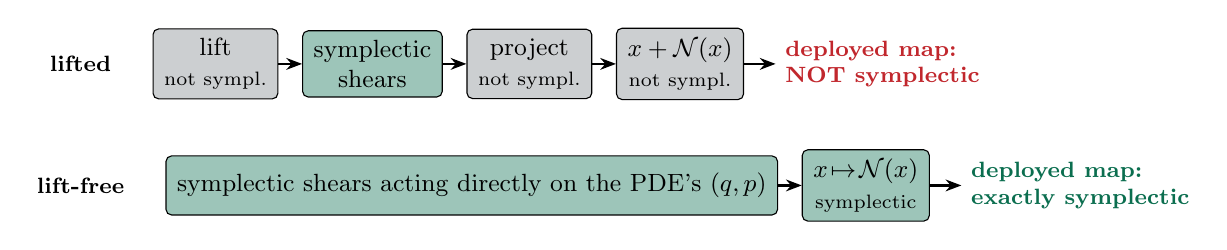
\begin{tikzpicture}[
  font=\small,
  box/.style={draw,rounded corners=2pt,minimum height=7.5mm,inner xsep=4pt,align=center},
  ar/.style={-{Stealth[length=2mm]},thick}
]
% lifted row
\node[font=\bfseries\footnotesize] (l1) {lifted};
\node[box,fill=cGrey!35,right=4mm of l1] (a1) {lift\\\scriptsize not sympl.};
\node[box,fill=cUnif!40,right=3mm of a1] (a2) {symplectic\\shears};
\node[box,fill=cGrey!35,right=3mm of a2] (a3) {project\\\scriptsize not sympl.};
\node[box,fill=cGrey!35,right=3mm of a3] (a4) {$x+\mathcal{N}(x)$\\\scriptsize not sympl.};
\node[right=4mm of a4,text=cCheb,font=\footnotesize\bfseries,align=left]
     (v1) {deployed map:\\NOT symplectic};
\draw[ar] (a1)--(a2); \draw[ar] (a2)--(a3); \draw[ar] (a3)--(a4); \draw[ar] (a4)--(v1);
% lift-free row
\node[font=\bfseries\footnotesize,below=11mm of l1] (l2) {lift-free};
\node[box,fill=cUnif!40,right=4mm of l2,minimum width=46mm] (b1)
     {symplectic shears acting directly on the PDE's $(q,p)$};
\node[box,fill=cUnif!40,right=3mm of b1] (b2) {$x\!\mapsto\!\mathcal{N}(x)$\\\scriptsize symplectic};
\node[right=4mm of b2,text=cUnif,font=\footnotesize\bfseries,align=left]
     (v2) {deployed map:\\exactly symplectic};
\draw[ar] (b1)--(b2); \draw[ar] (b2)--(v2);
\end{tikzpicture}
\caption{Where the guarantee is lost. The conventional wrapper surrounds a
symplectic core with three maps that are not symplectic; the composition
therefore carries no guarantee. \S\ref{sec:long} shows this is not a technicality:
at $2\times10^{4}$ steps the lifted variants diverge while the lift-free ones stay
bounded.}
\label{fig:lift}
\end{figure}

\subsection{The variants, and why each exists}

\begin{table}[htbp]
\centering
\caption{The operator variants compared, and the question each isolates.}
\label{tab:variants}
\small
\begin{tabular}{@{}p{33mm}lp{56mm}@{}}
\toprule
variant & symplectic in & role \\
\midrule
\texttt{sacheb} & $\Wc$ (core only) & Chebyshev-form gradient shear, lifted \\
\texttt{sacheb\_naive} & $\Wu$ (core only) & identical but uniform-form: isolates \emph{which} form \\
\texttt{sacheb\_pure} & $\Wc$ (end to end) & removes the lift: isolates \emph{where} the guarantee holds \\
\texttt{sacheb\_pure\_naive} & $\Wu$ (end to end) & both controls at once; the matched-form, fully-guaranteed operator \\
\ckino{} & neither & the non-gradient kernel; volume-preserving only \\
\ckino{}-strict & neither & exactly-constrained variant of \ckino{} \\
\ckino{}-nosymp & n/a & structure removed: isolates the block's contribution \\
SNO \citep{makara2026sno} & $\Wu$ (core only) & Fourier symplectic reference \\
FNO, T-FNO, U-FNO, U-Net, DeepONet, Transformer & n/a & unstructured references \\
GENERIC-FNO \citep{sulskis2026generic} & metriplectic & dissipative reference (see \S\ref{sec:limits}) \\
\bottomrule
\end{tabular}
\end{table}

Table~\ref{tab:variants} lists the comparison. The design is a $2\times2$ factorial, $\{$Chebyshev, Fourier$\}$ basis $\times$ $\{$symplectic, not$\}$,
realised as \sacheb{}/\ckino{}/SNO/FNO, crossed with two further controls that
vary \emph{which} form is preserved and \emph{whether the deployed map} preserves
it.

% ============================================================================
\section{Measuring structure: the symplectic defect}
\label{sec:defect}
% ============================================================================

Proposition~\ref{prop:shear} turns the question into a number. For a shear field
$F$ we form $A=DF$ by reverse-mode differentiation and report
\begin{equation}
\defect_W(F) \;=\; \frac{\lVert WA-A^{\top}W\rVert_F}{\lVert WA\rVert_F},
\label{eq:defect}
\end{equation}
zero iff the block preserves $\omega_W$. Crucially we evaluate
\eqref{eq:defect} for \emph{both} $W\in\{\Wc,\Wu\}$; reporting one column is what
produced the erroneous conclusion of our earlier draft.

\paragraph{Scaling to 3-D.} A dense Jacobian costs one backward pass per degree
of freedom, which is affordable at $N=32$ in $1$-D and hopeless at $16^3$.
Proposition~\ref{prop:hutch} replaces it with a probe estimator whose
\emph{number} of automatic-differentiation passes does not grow with the grid.

\begin{proposition}[Probe estimators for the squared norms]
\label{prop:hutch}
Let $M_\ast := WA-A^{\top}W$ and let $v\sim\mathcal{N}(0,I)$. Then
\begin{equation}
M_\ast v \;=\; W(Av)\;-\;A^{\top}(Wv),
\qquad
\mathbb{E}_v\big[\lVert M_\ast v\rVert^2\big] \;=\; \lVert M_\ast\rVert_F^2 ,
\label{eq:hutch}
\end{equation}
so averaging $\lVert M_\ast v\rVert^2$ over $m$ independent probes is an unbiased
estimator of $\lVert M_\ast\rVert_F^2$, and the same argument applied to $WA$ is
unbiased for $\lVert WA\rVert_F^2$. Each probe costs one Jacobian--vector product
($Av$) and one vector--Jacobian product ($A^{\top}u$), so the \emph{number} of
differentiation passes is $2m$ whatever the state dimension.
\end{proposition}

\begin{proof}
The first identity is linearity: $(WA-A^{\top}W)v=W(Av)-A^{\top}(Wv)$, and the two
terms are exactly a JVP and a VJP of the shear field, so neither requires $A$ to
be formed. For the second, $\mathbb{E}[vv^{\top}]=I$ gives
\[
\mathbb{E}_v\big[\lVert M_\ast v\rVert^2\big]
= \mathbb{E}_v\big[v^{\top}M_\ast^{\top}M_\ast v\big]
= \mathrm{tr}\big(M_\ast^{\top}M_\ast\,\mathbb{E}[vv^{\top}]\big)
= \mathrm{tr}\big(M_\ast^{\top}M_\ast\big)
= \lVert M_\ast\rVert_F^2 .
\]
The same argument applied to $WA$ estimates the denominator of
\eqref{eq:defect}, so the ratio is formed from two estimates sharing the JVP.
\end{proof}

\begin{remark}[What is unbiased, and what the estimator costs]
\label{rem:ratio}
Proposition~\ref{prop:hutch} is unbiased for the two \emph{squared} norms, not
for their ratio. What we report is
\begin{equation}
\widehat{\defect}_W
=\left(\frac{\sum_{i=1}^{m}\lVert M_\ast v_i\rVert^2}
            {\sum_{i=1}^{m}\lVert WAv_i\rVert^2}\right)^{1/2},
\label{eq:ratio-est}
\end{equation}
a ratio of square roots of two unbiased estimates. This is consistent as
$m\to\infty$ but is not itself unbiased, and we do not claim otherwise;
numerator and denominator share probes, which cancels part of the $O(1/m)$
bias. Two accounting points are worth stating plainly, because it would be easy
to overclaim both. First, what is independent of the grid is the \emph{number}
of differentiation passes, $2m$ rather than one per degree of freedom; the
runtime of each pass still scales with the cost of evaluating the operator,
$O(RN^d)$ for the low-rank kernel of \S\ref{sec:sacheb}. The saving is a factor
of $N^d/2m$ in passes, not a constant-time measurement. Second, the estimator is
stochastic, so the $O(1)$ off-diagonal entries of Figure~\ref{fig:defect} carry
probe noise; the machine-precision diagonal does not, since a genuinely
symplectic block returns zero for every probe.
\end{remark}

We use $m=96$ probes. Against the dense path the estimator agrees to $\le7\%$ on
$O(1)$ values and correctly returns machine zero; the dense path is retained
wherever the state has at most $1200$ degrees of freedom, and is what the
estimator is validated against.

% ============================================================================
\section{Experimental protocol}
\label{sec:setup}
% ============================================================================

\subsection{The physical systems}
\label{sec:systems}

Nine equations span two axes that matter for structure preservation: linear
versus nonlinear, and conservative versus dissipative. Four of them are
Hamiltonian in a canonical $(q,p)=(u,\partial_t u)$ pair, which is the subset on
which a symplectic construction is meaningful at all; the remaining five are
scalar fields, where no canonical splitting exists and the lift-free variants of
\S\ref{sec:lift} cannot be run. Table~\ref{tab:systems} gives the full
specification.

\begin{table}[htbp]
\centering
\caption{The nine systems. $L=2$ throughout except \texttt{wave1d\_dir}, where
$L=1$. ``Sub'' counts solver micro-steps per stored step. The four two-field
systems are the ones carrying a canonical $(q,p)$ pair, and therefore the only
ones on which the lift-free operators of \S\ref{sec:lift} can act.}
\label{tab:systems}
\footnotesize
\setlength{\tabcolsep}{4pt}
\begin{tabular}{llllrl}
\toprule
Problem & Equation & Domain, boundary & Grid & $\Delta t$ & Reference integrator \\
\midrule
\multicolumn{6}{l}{\emph{Scalar fields: one channel, no canonical $(q,p)$ pair}}\\
\texttt{advection} & $u_t+cu_x=0$, $c=1$ & $[-1,1)$, periodic & $64$ & $0.005$ & exact spectral \\
\texttt{heat} & $u_t=\nu u_{xx}$, $\nu=10^{-2}$ & $[-1,1)$, periodic & $64$ & $0.005$ & exact spectral \\
\texttt{burgers} & $u_t+uu_x=\nu u_{xx}$, $\nu=2\!\times\!10^{-2}$ & $[-1,1)$, periodic & $64$ & $0.005$ & ETD-RK2, $8$ sub \\
\texttt{kdv} & $u_t+6uu_x-u_{xxx}=0$ & $[-1,1)$, periodic & $64$ & $10^{-3}$ & pseudo-spectral, $10$ sub \\
\texttt{ns2d} & $w_t+(\mathbf{u}\!\cdot\!\nabla)w=\nu\Delta w$, $\nu=3\!\times\!10^{-3}$ & $[-1,1)^2$, periodic & $64^2$ & $0.01$ & ETD-RK2, $2/3$ dealiased, $4$ sub \\
\midrule
\multicolumn{6}{l}{\emph{Hamiltonian: two channels $(u,v)$, $v=\partial_t u$}}\\
\texttt{wave1d} & $u_{tt}=c^2u_{xx}$, $c=1$ & $[-1,1)$, periodic & $32$ & $0.02$ & leap-frog, $4$ sub \\
\texttt{wave1d\_dir} & $u_{tt}=c^2u_{xx}$, $c=1$ & $[0,1]$, Dirichlet & $64$ & $0.005$ & leap-frog, $4$ sub \\
\texttt{wave2d} & $u_{tt}=c^2\Delta u$, $c=1$ & $[-1,1)^2$, periodic & $32^2$ & $0.02$ & leap-frog, $4$ sub \\
\texttt{wave3d} & $u_{tt}=c^2\Delta u$, $c=1$ & $[-1,1)^3$, periodic & $16^3$ & $0.02$ & leap-frog, $4$ sub \\
\bottomrule
\end{tabular}
\end{table}

\paragraph{What each one tests.} \texttt{advection} is pure transport: linear,
non-dispersive, and conserving both $\int u$ and $\int u^2$, so it is the floor
below which a surrogate has no excuse. \texttt{heat} is linear but strictly
dissipative, which makes it a control: energy decay is the correct behaviour, so
a model that artificially conserves energy is penalised rather than rewarded.
\texttt{burgers} adds nonlinearity to dissipation and steepens into shock
fronts, testing whether a spectral parameterisation can represent a sharp front
without Gibbs oscillation. \texttt{kdv} is the nonlinear dispersive case, with
soliton interaction and a conserved Hamiltonian
$\mathcal{H}=\int(u_x^2-2u^3)\,dx$; its $\Delta t=10^{-3}$ and ten micro-steps
reflect the stiff $u_{xxx}$ term. \texttt{ns2d} is decaying two-dimensional
turbulence in vorticity form, the canonical neural-operator benchmark, and the
only problem here with a genuine energy cascade.

The four wave problems carry the conserved Hamiltonian
$\mathcal{H}=\tfrac12\int(v^2+c^2\lVert\nabla u\rVert^2)$ and are integrated by
St\"ormer--Verlet leap-frog, so the reference trajectories are themselves
symplectic. This matters for interpreting \S\ref{sec:long}: when we ask whether
a learned operator conserves energy over $2\times10^{4}$ steps, the ground truth
against which it is compared does so by construction.

\texttt{wave1d\_dir} is the discriminating rung. It is the wave equation on
$[0,L]$ with homogeneous \emph{Dirichlet} boundaries, a uniform grid, centred
differences and symplectic leap-frog, with initial conditions formed from a
truncated Chebyshev series times the envelope $x(L-x)$. This mirrors the
data-generation protocol of \citet{makara2026sno}, so the comparison is made on
the concurrent method's own terms. It is simultaneously Hamiltonian, so
symplecticity is meaningful, and non-periodic, so a Fourier parameterisation is
structurally mismatched. The reference solver conserves energy to
$2.3\times10^{-4}$ over $500$ steps and holds the boundary at exactly zero.

\subsection{Nodes, representation and quadrature in each experiment}
\label{sec:nodes}

The theory of \S\ref{sec:background} is posed on CGL nodes, where the
Clenshaw--Curtis weights are the correct quadrature. The experiments are not:
every dataset in Table~\ref{tab:systems} is sampled on a uniform grid.
Table~\ref{tab:nodes} states exactly what this means for each run, because the
paper's central claim is that the inner product must match the discretisation,
and a reader cannot check that claim without knowing which nodes carry which
weights.

\begin{table}[htbp]
\centering
\caption{Nodes and quadrature. The operator stores its basis as Chebyshev
coefficients and evaluates them on the CGL grid of matching size, so sample
index $j$ is read as the node $x_j=\cos(j\pi/N)$ regardless of where the
datum was actually sampled. Because all physical grids are uniform, $\Wu$ is
the matched form in every one of the nine experiments; the converse
configuration is not tested here (\S\ref{sec:limits}).}
\label{tab:nodes}
\footnotesize
\setlength{\tabcolsep}{5pt}
\begin{tabular}{lllll}
\toprule
Dataset & Physical nodes & Model reads them as & Physical quadrature & Matched form \\
\midrule
\texttt{advection}  & $64$ uniform      & $64$ CGL   & constant $L/N$ & $\Wu$ \\
\texttt{heat}       & $64$ uniform      & $64$ CGL   & constant $L/N$ & $\Wu$ \\
\texttt{burgers}    & $64$ uniform      & $64$ CGL   & constant $L/N$ & $\Wu$ \\
\texttt{kdv}        & $64$ uniform      & $64$ CGL   & constant $L/N$ & $\Wu$ \\
\texttt{wave1d}     & $32$ uniform      & $32$ CGL   & constant $L/N$ & $\Wu$ \\
\texttt{wave1d\_dir}& $64$ uniform      & $64$ CGL   & constant $L/N$ & $\Wu$ \\
\texttt{wave2d}     & $32^2$ uniform    & $32^2$ CGL & constant $(L/N)^2$ & $\Wu$ \\
\texttt{wave3d}     & $16^3$ uniform    & $16^3$ CGL & constant $(L/N)^3$ & $\Wu$ \\
\texttt{ns2d}       & $64^2$ uniform    & $64^2$ CGL & constant $(L/N)^2$ & $\Wu$ \\
\bottomrule
\end{tabular}
\end{table}

Concretely, $\Wc=\mathrm{diag}(w_0,\dots,w_N)$ holds the Clenshaw--Curtis
weights for the $N+1$ CGL nodes, and $\Wu=\tfrac{2}{N+1}I$ holds constant
weights; in $d$ dimensions each is the outer product of its per-axis factor. The
two enter at exactly one place, the adjoint $K^{*}=W^{-1}K^{\top}W$ of
\eqref{eq:adjoint}, and nowhere else. Everything else about the two operators,
including the Chebyshev basis, the rank, the channel mixing and the
initialisation, is identical.

The consequence is worth stating bluntly, since it bounds what the experiments
can establish. Because every physical grid is uniform, $\Wu$ is the matched form
throughout and $\Wc$ is the mismatched one throughout. The ablation of
\S\ref{sec:ablation} therefore tests the matching hypothesis in one direction
only. It shows that the mismatched form loses; it cannot by itself separate
``matching the form to the grid is what matters'' from ``constant weights are
simply the better choice''. Distinguishing those requires a dataset genuinely
sampled on CGL nodes, where $\Wc$ becomes the matched form and the preference
should reverse. We have not run that experiment, and we regard it as the single
most important missing control in this study (\S\ref{sec:limits}).

\subsection{Data, splits and selection}
\label{sec:splits}

Trajectories are generated from random initial conditions with \emph{disjoint
seed ranges} per split, so no initial condition appears in more than one split.
Each $1$-D problem uses $512$ training trajectories of $600$ steps and is trained
for $15$ epochs; \texttt{wave2d} and \texttt{ns2d} use $96$ trajectories of $300$
steps ($15$ epochs), and \texttt{wave3d} uses $48$ trajectories of $200$ steps
($12$ epochs). Every problem has $12$ validation and $12$ test trajectories.
The data seeds are fixed independently of the training seed, so every model and
every seed is scored on the \emph{same} test trajectories; the three training
seeds vary only initialisation and minibatch order. Rollout metrics are always
computed on the test split, and are evaluated once.

One caveat applies to Table~\ref{tab:winners} specifically. The best
configuration per problem is chosen by comparing test-split rollout error across
all configurations, not by validation. Selecting the maximum of many noisy
scores biases that maximum optimistically, so the per-problem winners should be
read as an upper estimate rather than an unbiased one. The comparisons the
paper's claims actually rest on are not exposed to this: the form ablation
(\S\ref{sec:ablation}), the lift-free contrast (\S\ref{sec:long}), the defect
matrix (\S\ref{sec:form}) and the long-horizon rollouts are all \emph{pre-specified
paired} comparisons between two variants that differ in one design decision, with
no selection over a pool.

\subsection{Design, matching and cost}
\label{sec:design}

Families are crossed with prediction mode
$\{$recursive, non-recursive \texttt{seq2seq}$\}$, training noise
$\{$none, $2\%\}$ and an optional PDE-residual loss, giving $33$ configurations
in $1$-D and $21$ in $2$-D/$3$-D, all matched to $\approx$25k parameters. Three
seeds on a single hardware (NVIDIA Tesla T4): \textbf{783 training runs}.

Parameter count is the matching criterion, and it is the weakest of the
available ones. The families compared here have very different arithmetic
profiles at equal parameter count: a Fourier layer spends its budget on
multipliers applied through an FFT of cost $O(N^d\log N)$, a low-rank integral
kernel on $O(RN^d)$ contractions, attention on a quadratic term in sequence
length, and a U-Net on convolutions across a resolution hierarchy. Autoregressive
rollout multiplies all of these by the number of steps, while the
\texttt{seq2seq} variants pay once. Equal parameters therefore does not mean
equal memory, equal FLOPs or equal wall-clock, and none of the accuracy
comparisons in \S\ref{sec:accuracy} should be read as statements about
efficiency. Measured throughput is reported separately in \S\ref{sec:support},
where the spread is roughly an order of magnitude.

\paragraph{Metrics.} Relative RMS at rollout checkpoints, plus amplitude ratio,
pattern correlation, spectral error and invariant drift, collapsed into a
\emph{verdict} and a \emph{usable horizon} (last step with correlation $\ge0.9$
and amplitude ratio in $[0.7,1.4]$). A model can post a middling RMS while being
physically dead, and only the decomposition separates the two.

% ============================================================================
\section{Results}
% ============================================================================

\subsection{Which form does each construction preserve?}
\label{sec:form}

\begin{figure}[htbp]
\centering
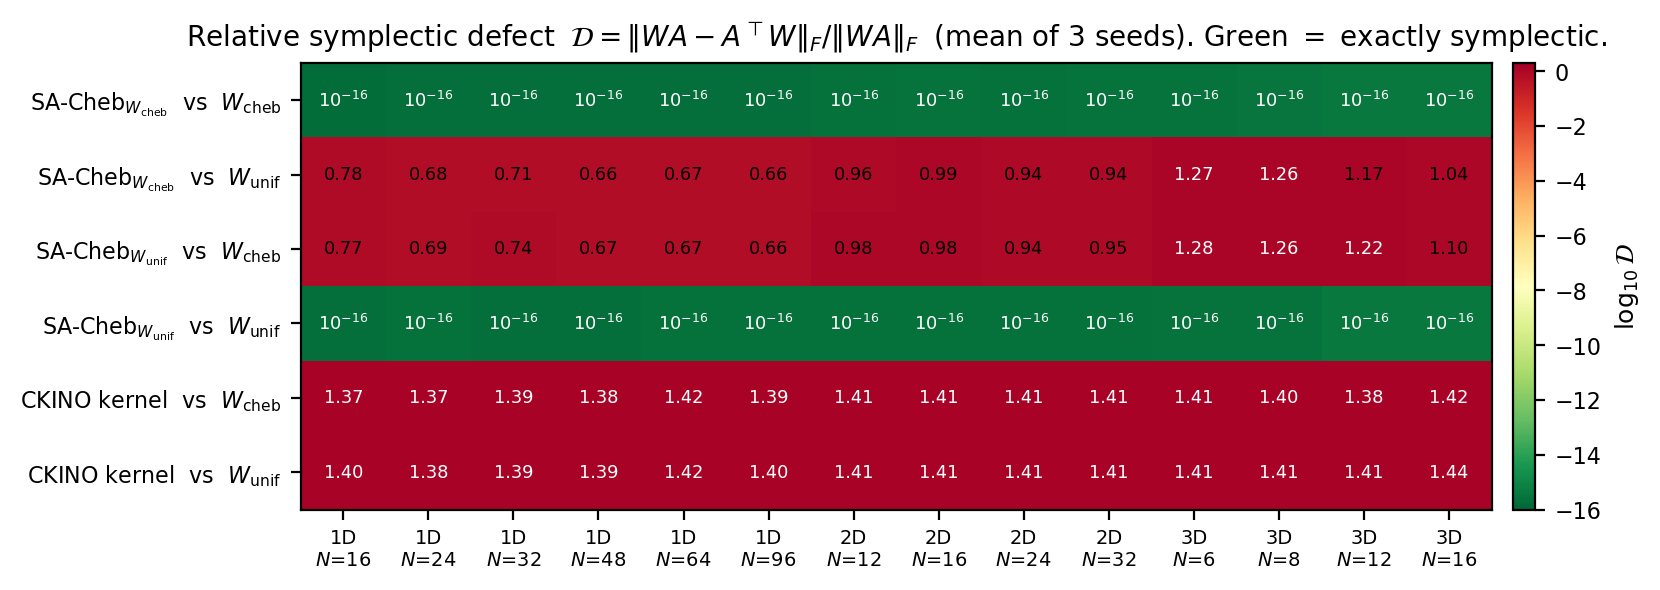
\includegraphics[width=\linewidth]{figs/defect_matrix.png}
\caption{Symplectic defect of every construction against \emph{both} inner
products, over $14$ grid configurations in $1$-D, $2$-D and $3$-D, mean of three
seeds. The green diagonal is the result: each gradient shear is exact in the form
its adjoint was built from and $O(1)$ in the other. The \ckino{} kernel is $\approx1.4$ in both: volume-preserving, not symplectic.}
\label{fig:defect}
\end{figure}

Figure~\ref{fig:defect} is the central measurement. Three conclusions follow.

\textbf{(i)} Theorem~\ref{thm:sacheb} holds numerically: $2$--$4\times10^{-16}$,
independent of resolution and dimension. \textbf{(ii)} The two variants are
\emph{both} exactly symplectic, in different forms; neither is ``broken''. The
off-diagonal grows with dimension ($\approx0.7$ in $1$-D, $\approx0.95$ in $2$-D,
$1.0$--$1.3$ in $3$-D) because the tensor-product weight varies more.
\textbf{(iii)} The \ckino{} kernel is $\approx1.4$ in both forms, exactly the
conflation flagged in Remark~\ref{rem:volume}.

\subsection{Does the choice of form matter?}
\label{sec:ablation}

Every benchmark here is discretised on a \emph{uniform} grid, so $\Wu$ is the
physically relevant form and $\Wc$ is not. Figure~\ref{fig:ablation} compares
models that are identical in architecture, parameter count and training recipe
and differ only in the adjoint.

\begin{figure}[htbp]
\centering
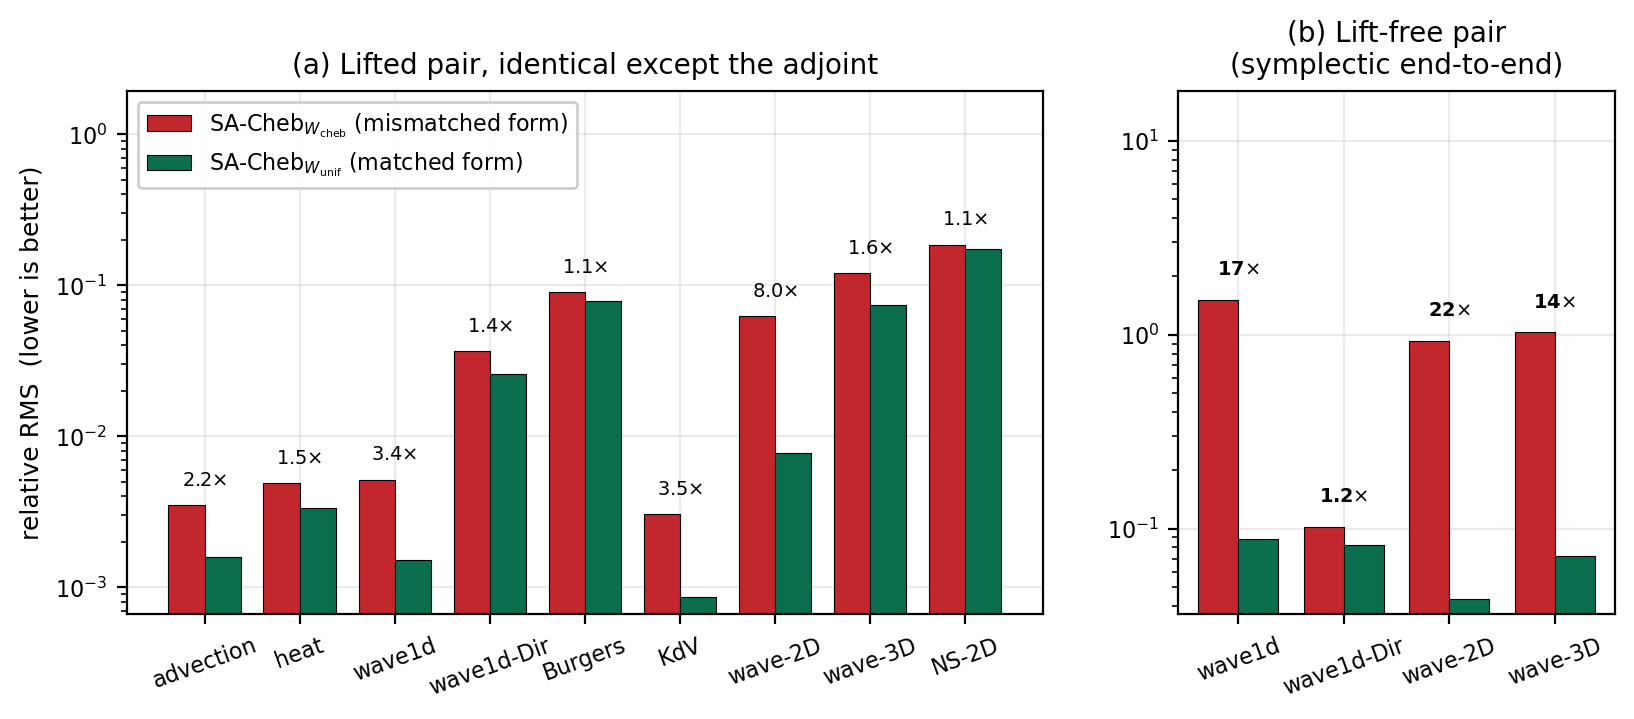
\includegraphics[width=\linewidth]{figs/form_ablation.png}
\caption{Matched-form versus mismatched-form at identical capacity (3 seeds).
\textbf{(a)} Lifted pair: the matched-form model wins every problem, by
$1.1$--$8.0\times$. \textbf{(b)} Lift-free pair, where the deployed map really is
symplectic: the margin widens to $14$--$22\times$. Removing the non-symplectic
wrapper does not just help; it amplifies the effect of getting the form right by
an order of magnitude.}
\label{fig:ablation}
\end{figure}

Over the full matrix the matched-form model wins \textbf{16 of 18} paired
comparisons (the two exceptions are a tie at the divergence clip and a $1.04\times$
gap inside one standard deviation). For the lift-free pair it is $4/4$.

\begin{table}[htbp]
\centering
\caption{Lift-free pair: both models exactly symplectic \emph{end to end},
differing only in which form. Relative RMS, 3 seeds.}
\label{tab:pure}
\small
\begin{tabular}{@{}lccc@{}}
\toprule
problem & \texttt{purecheb} ($\Wc$) & \texttt{pureunif} ($\Wu$) & ratio \\
\midrule
\texttt{wave1d}      & 1.5182 & \textbf{0.08809} & $17.2\times$ \\
\texttt{wave1d\_dir} & 0.1020 & \textbf{0.08242} & $1.24\times$ \\
\texttt{wave2d}      & 0.9332 & \textbf{0.04316} & $21.6\times$ \\
\texttt{wave3d}      & 1.0273 & \textbf{0.07238} & $14.2\times$ \\
\bottomrule
\end{tabular}
\end{table}

\subsection{Long-horizon behaviour: the lift is decisive}
\label{sec:long}

\begin{figure}[htbp]
\centering
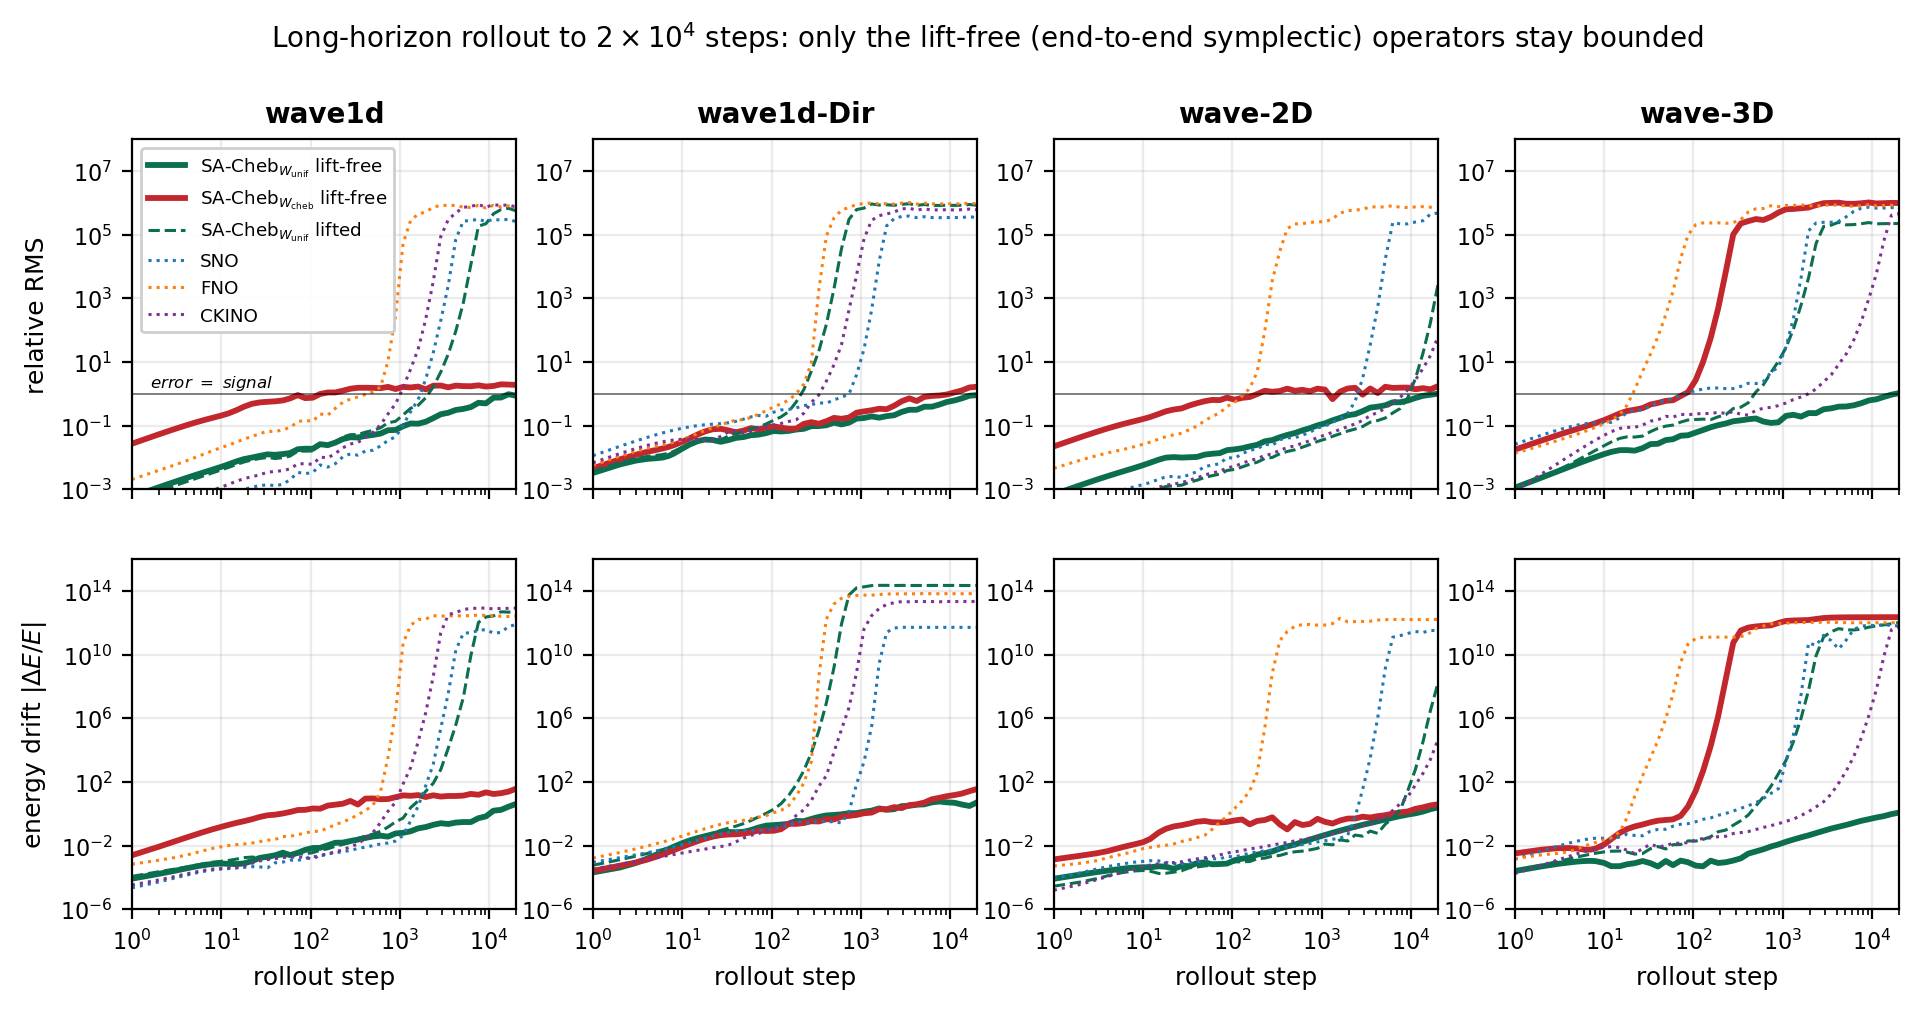
\includegraphics[width=\linewidth]{figs/longhorizon.png}
\caption{Rollout to $2\times10^{4}$ steps, mean of 3 seeds. \textbf{Top:}
relative error; the thin line marks error $=$ signal. \textbf{Bottom:} energy
drift on the model's own trajectory. Every lifted or unstructured operator, whether FNO, SNO, \ckino{} or the lifted \sacheb{} variants, leaves the solution manifold
and reaches $10^{5}$--$10^{12}$. The lift-free operators stay bounded. The
matched-form lift-free model (green) is bounded on all four problems; the
mismatched-form one (red) survives three of four.}
\label{fig:long}
\end{figure}

This is the study's strongest result and it was not visible at the few-hundred-step
horizon of the main matrix. Figure~\ref{fig:long} and Table~\ref{tab:long} show
that in these experiments exact \emph{end-to-end} symplecticity is associated
with bounded trajectories and with energy drift of order unity, while nothing
else in the comparison stays on the solution manifold at all.

Two qualifications belong with that sentence. The first is theoretical.
Backward-error analysis explains why symplectic \emph{integrators} conserve a
modified Hamiltonian over exponentially long times \citep{hairer2006gni}, but it
assumes a consistent approximation to a specified flow at small step size, and
builds a modified equation from exactly those hypotheses. A learned operator
satisfies none of them merely by having a symplectic Jacobian: it is not a
discretisation of a known Hamiltonian at small $\Delta t$, and no modified
Hamiltonian is available to appeal to. What we observe is consistent with the
qualitative motivation of geometric integration, and we report it on that
footing; it is not an instance of the theorem.

The second concerns what boundedness actually buys. A relative RMS between
$0.87$ and $1.05$ is bounded, and it is also an error comparable to the signal
itself: these models are not tracking the reference trajectory at step
$2\times10^{4}$. What survives is the amplitude and the qualitative character of
the field rather than its phase. The defensible statement is that the lift-free
symplectic variants remain numerically bounded and physically plausible while
every alternative leaves the manifold by five to twelve orders of magnitude, and
that boundedness at this horizon is a different property from predictive
accuracy. Figures~\ref{fig:fields-dir} and~\ref{fig:fields-long} show the
distinction directly.

\begin{table}[htbp]
\centering
\caption{State at step $2\times10^{4}$ (mean of 3 seeds). Bold rows are bounded;
the rest have left the solution manifold entirely.}
\label{tab:long}
\small
\begin{tabular}{@{}llcc@{}}
\toprule
problem & family & relative RMS & energy drift $|\Delta E/E|$ \\
\midrule
\multirow{3}{*}{\texttt{wave1d}}
 & \textbf{pureunif (lift-free, $\Wu$)} & \textbf{0.868} & \textbf{4.18} \\
 & \textbf{purecheb (lift-free, $\Wc$)} & \textbf{1.902} & \textbf{37.9} \\
 & SNO / FNO / lifted \sacheb{} & $2.6$--$7.2\times10^{5}$ & $10^{11}$--$10^{12}$ \\
\midrule
\multirow{3}{*}{\texttt{wave1d\_dir}}
 & \textbf{pureunif} & \textbf{0.908} & \textbf{5.24} \\
 & \textbf{purecheb} & \textbf{1.659} & \textbf{36.2} \\
 & SNO / FNO & $3.4$--$9.4\times10^{5}$ & $10^{11}$--$10^{13}$ \\
\midrule
\multirow{3}{*}{\texttt{wave2d}}
 & \textbf{pureunif} & \textbf{1.008} & \textbf{2.52} \\
 & \textbf{purecheb} & \textbf{1.739} & \textbf{3.94} \\
 & FNO & $7.3\times10^{5}$ & $1.7\times10^{12}$ \\
\midrule
\multirow{2}{*}{\texttt{wave3d}}
 & \textbf{pureunif} & \textbf{1.047} & \textbf{1.19} \\
 & SNO / FNO / lifted & $2.8$--$8.3\times10^{5}$ & $10^{11}$--$10^{12}$ \\
\bottomrule
\end{tabular}
\end{table}

\begin{remark}[Read the slope with the error]
A drift exponent near zero is \emph{not} by itself evidence of health. FNO scores
$-0.02$ on \texttt{wave1d} while sitting at relative RMS $7\times10^{5}$: once the
state has blown up, the drift ratio saturates and its slope becomes meaningless.
\end{remark}

\paragraph{Independent corroboration.} \citet{sulskis2026generic} report the same
qualitative effect for the metriplectic case: over $200$-step rollouts, every
unconstrained model they test diverges or collapses while their
structure-preserving operator stays bounded. That two constructions enforcing
different structures (symplectic here, GENERIC there) both buy boundedness and
little else suggests the effect is a property of exact structure preservation
rather than of either particular bracket.

\paragraph{The same result seen as fields.} Figures~\ref{fig:fields-dir} and
\ref{fig:fields-long} show the rollout as the state itself rather than as summary
curves. They make two things visible that Figure~\ref{fig:long} cannot. First,
the failure modes are \emph{qualitatively different}: blow-up (the lifted
variants and FNO), amplitude collapse (SNO), and graceful roughening at preserved
amplitude (lift-free). Second, amplitude collapse produces a field that is
numerically well behaved, with no overflow and bounded norm, while carrying none of the
physics, which is precisely the case an RMS-only evaluation at short horizon
would pass.

\begin{figure}[htbp]
\centering
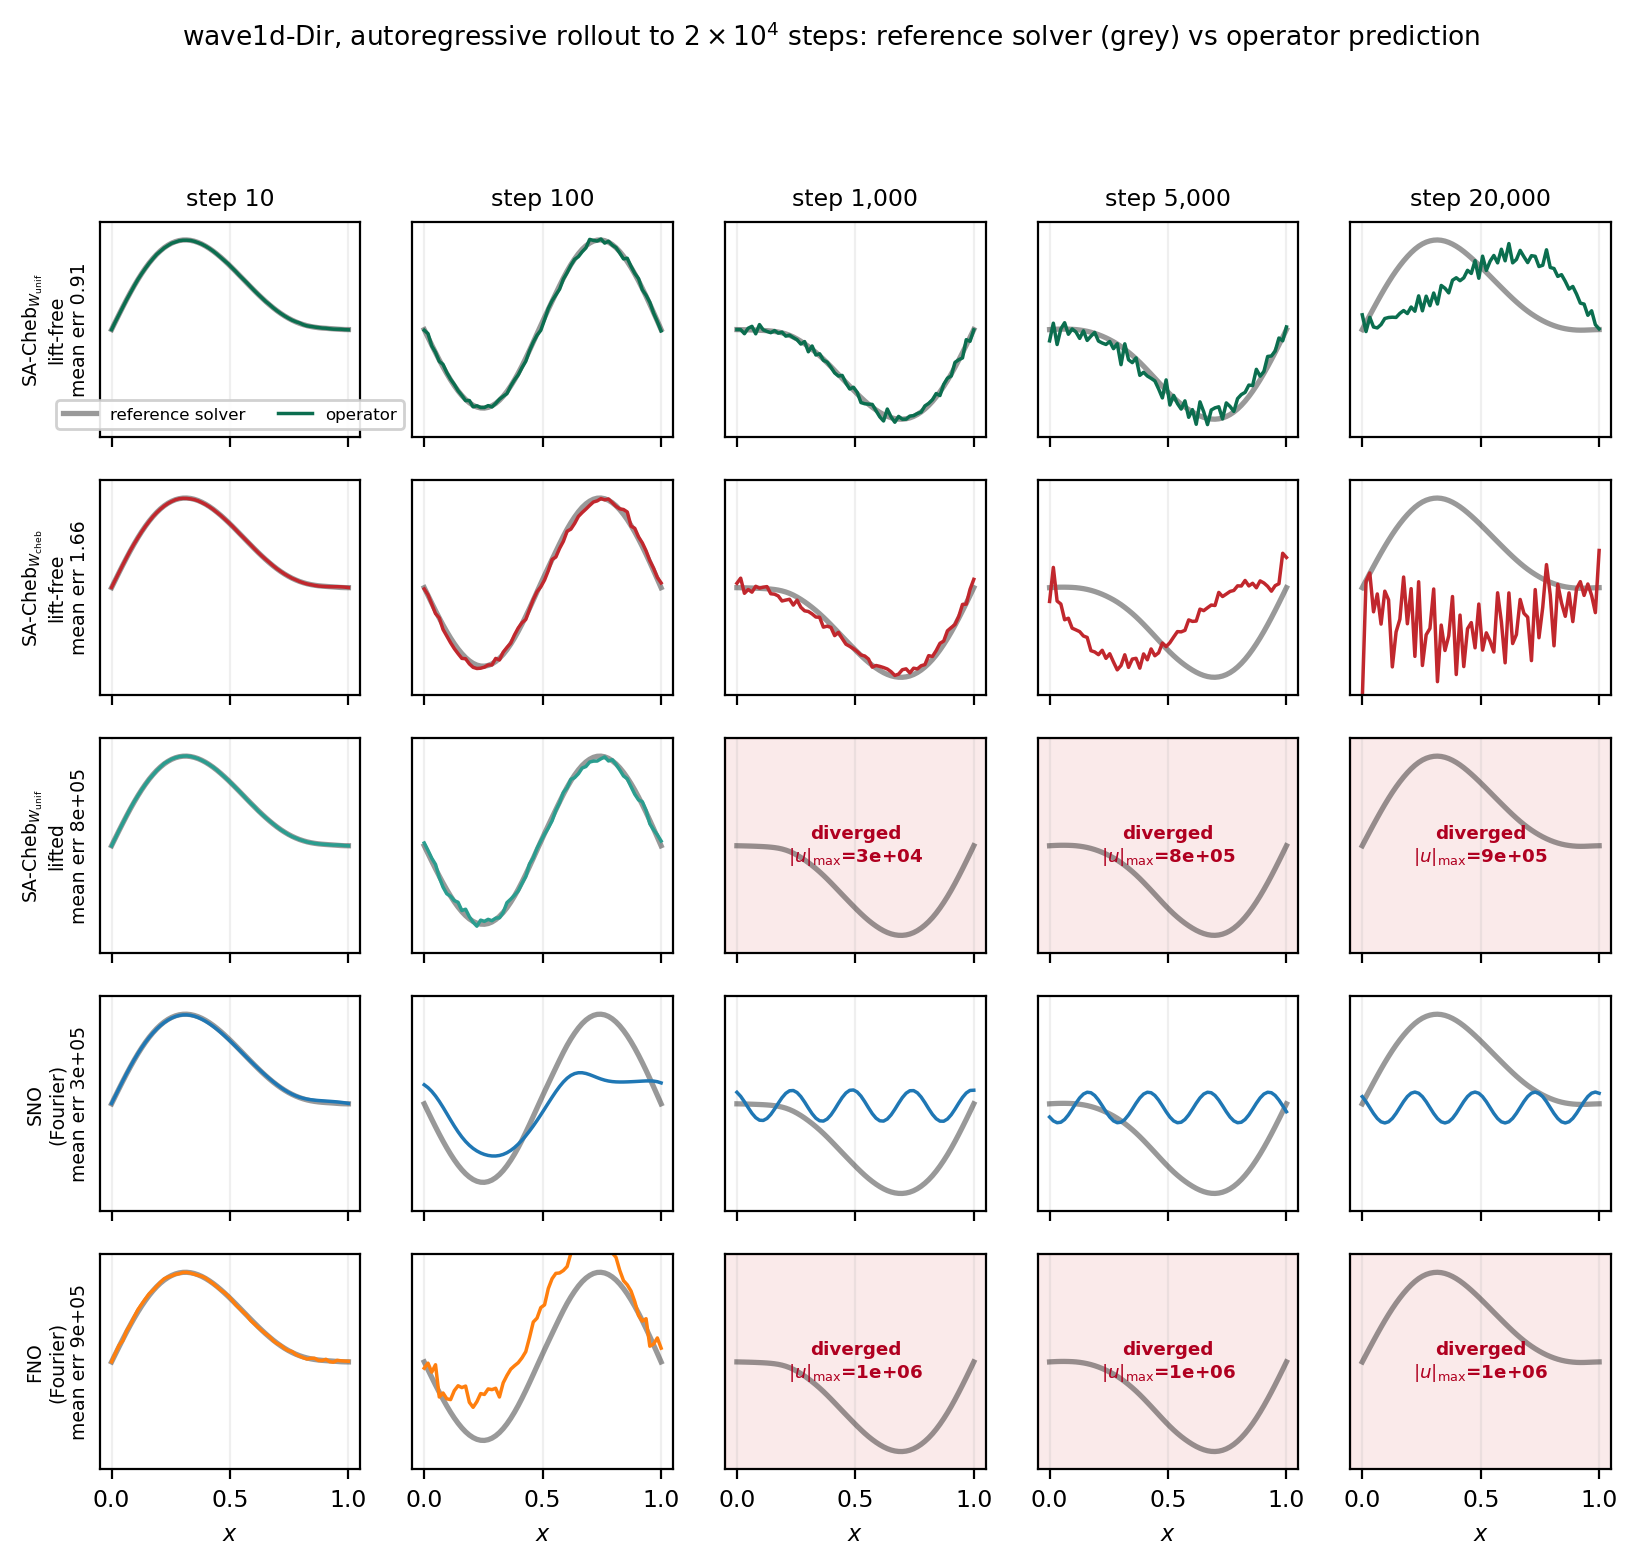
\includegraphics[width=\linewidth]{figs/timelapse_wave1d_dir.png}
\caption{\texttt{wave1d\_dir} time lapse over the $2\times10^{4}$-step rollout:
reference solver (grey) against operator prediction. Row labels carry each
family's population error over all test trajectories, so a single plotted
trajectory cannot be over-read. The \emph{lifted} SA-Cheb and FNO blow up; SNO
collapses to a low-amplitude oscillation that is bounded but carries none of the physics; only the \emph{lift-free} operators track the wave to $2\times10^{4}$
steps.}
\label{fig:fields-dir}
\end{figure}

\begin{figure}[htbp]
\centering
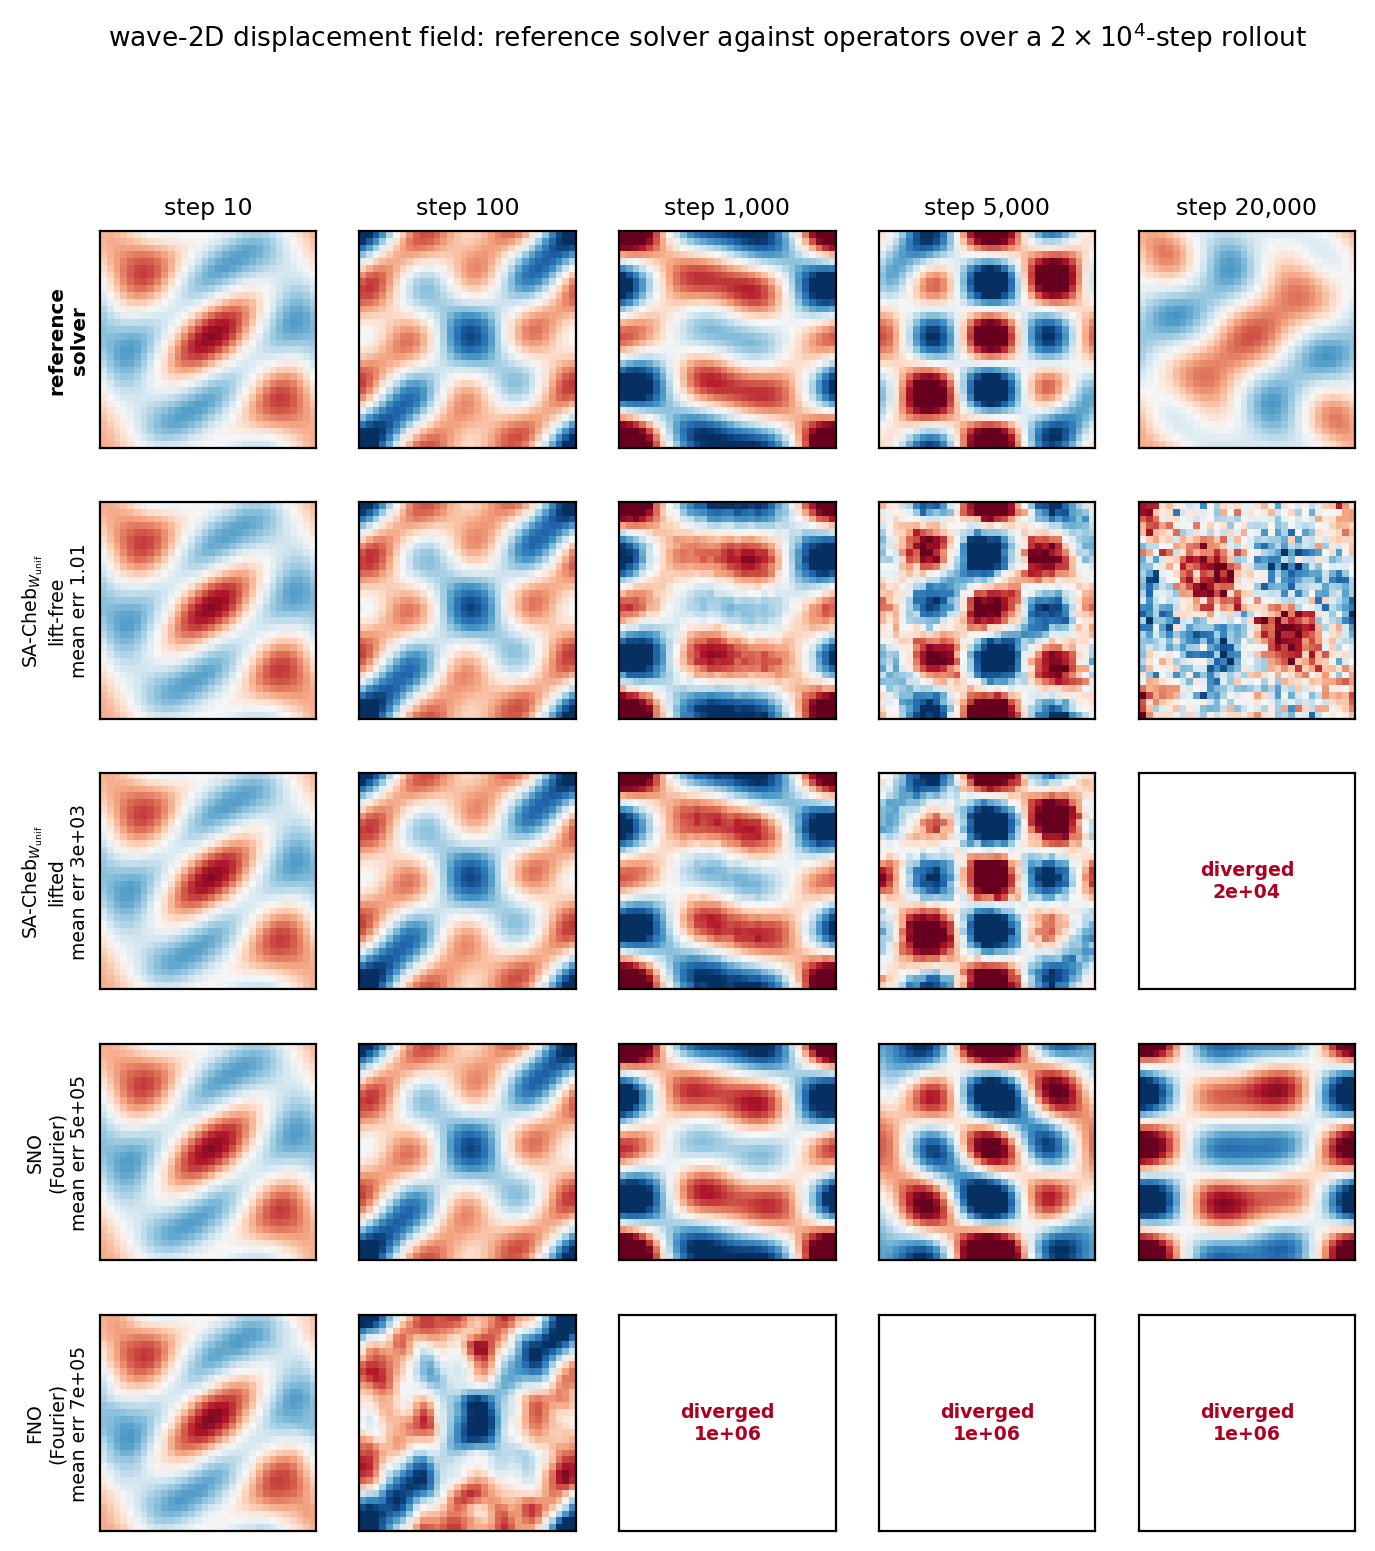
\includegraphics[width=\linewidth]{figs/timelapse_wave2d.png}
\caption{\texttt{wave2d} displacement field over the same rollout. The reference
solver sustains a coherent interference pattern throughout. The lift-free
matched-form operator degrades gracefully into noise while remaining bounded; the
\emph{lifted} variant, built from the same gradient-shear construction at the
same parameter budget, has diverged by $2\times10^{4}$, and FNO by $10^{3}$. The
two are matched on parameter \emph{count}, not built from identical tensors:
dropping the lift forces $H=C$, so the lift-free model must recover capacity
through rank and depth (\S\ref{sec:lift}).}
\label{fig:fields-long}
\end{figure}

\subsection{Basis versus boundary}
\label{sec:basis}

\begin{figure}[htbp]
\centering
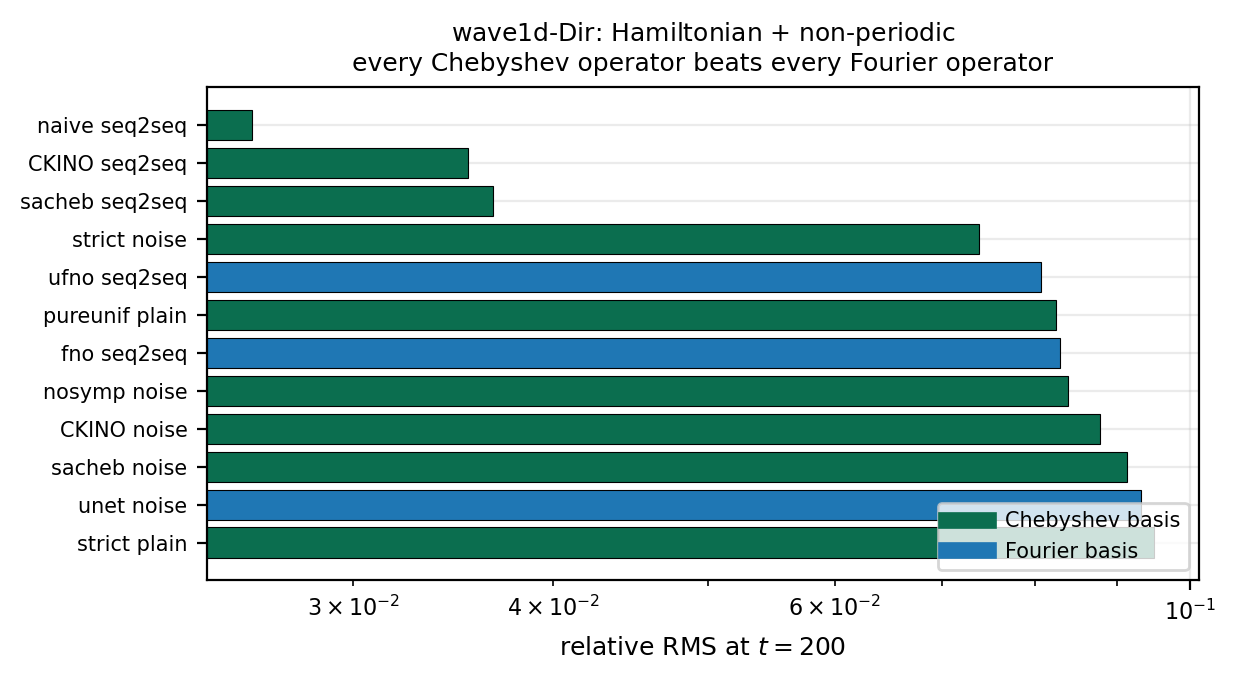
\includegraphics[width=0.72\linewidth]{figs/basis_boundary.png}
\caption{\texttt{wave1d\_dir}, the Hamiltonian non-periodic rung. Every Chebyshev
operator beats every Fourier operator: $3.2\times$ over the best FNO and
$6.5\times$ over SNO, on a benchmark built to match SNO's own data protocol. The
mechanism is the Gibbs penalty the Dirichlet envelope imposes on a periodic
basis.}
\label{fig:basis}
\end{figure}

The converse holds too, which is what makes this a rule rather than a cherry-pick:
in one dimension the winning basis follows the boundary conditions \emph{exactly}:
Fourier operators take all four periodic problems and the Chebyshev family
takes the one non-periodic problem, while the Chebyshev operator additionally
takes all three multi-dimensional problems. No structural prior is needed to
explain the split.

\subsection{Accuracy across the full matrix}
\label{sec:accuracy}

\begin{table}[htbp]
\centering
\caption{Best configuration per problem (relative RMS, mean $\pm$ std, 3 seeds).}
\label{tab:winners}
\small
\begin{tabular}{@{}llcl@{}}
\toprule
problem & best model & relative RMS & basis \\
\midrule
advection$^\ddagger$   & SNO (seq2seq)                   & $0.001196 \pm 0.00016$ & Fourier \\
heat                 & T-FNO (recursive)               & $0.001090 \pm 0.00031$ & Fourier \\
\texttt{wave1d}      & SNO (seq2seq)                   & $0.001103 \pm 0.00039$ & Fourier \\
\texttt{wave1d\_dir} & \texttt{sacheb\_naive} (seq2seq)& $0.025939 \pm 0.0021$  & Chebyshev \\
Burgers              & T-FNO (recursive)               & $0.003963 \pm 0.00098$ & Fourier \\
KdV                  & SNO (seq2seq)                   & $0.000511 \pm 0.000064$& Fourier \\
\texttt{wave2d}      & \texttt{sacheb\_naive} (seq2seq)& $0.007771 \pm 0.0015$  & Chebyshev \\
\texttt{wave3d}      & \texttt{pureunif} (recursive)   & $0.072375 \pm 0.0089$  & Chebyshev \\
\texttt{ns2d}        & \texttt{sacheb\_naive} (seq2seq)& $0.174500 \pm 0.0014$  & Chebyshev \\
\bottomrule
\end{tabular}

\vspace{2pt}
{\footnotesize $^\ddagger$ advection is a tie within seed noise: the contending
Chebyshev model varies by $15.7\times$ across seeds there, and the winner changed
between two executions of the study (\S\ref{sec:repro}). We do not claim it.}
\end{table}

\begin{figure}[htbp]
\centering
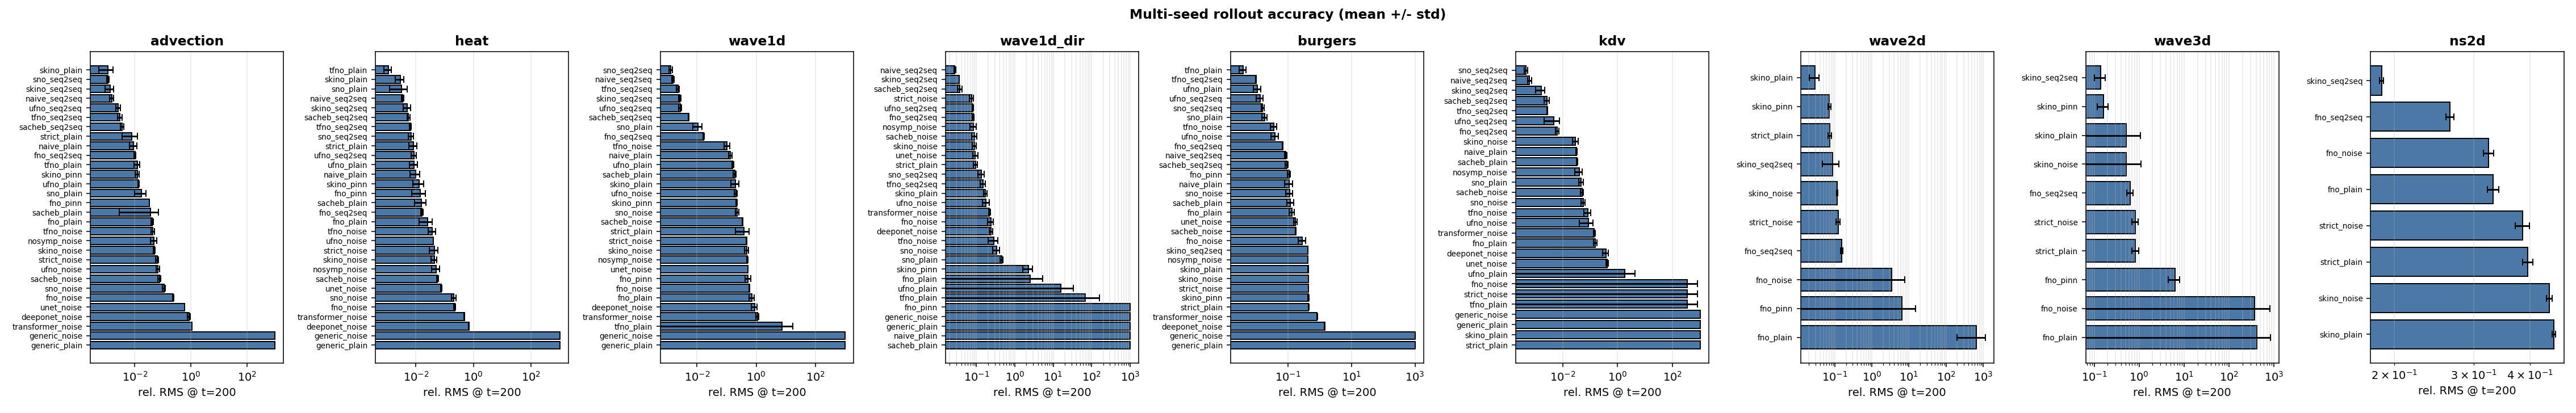
\includegraphics[width=\linewidth]{figs/multiseed.png}
\caption{Relative RMS (log scale, mean $\pm$ std over 3 seeds) for the best
twelve configurations per equation, all matched to $\approx$25k parameters. The
panel titles give the size of the pool each twelve is drawn from; the full
listing is in the released \texttt{summary.csv}. Note the horizontal scales
differ per panel: the spread within a problem ranges from under a decade
(\texttt{ns2d}) to more than two (\texttt{wave1d}).}
\label{fig:multiseed}
\end{figure}

Against the parameter-matched references the margins in higher dimensions are
$19.8\times$ over FNO on \texttt{wave2d}, $8.8\times$ over FNO and $4.8\times$
over SNO on \texttt{wave3d}, and $1.5\times$/$1.4\times$ on \texttt{ns2d}. We
stress that SNO is now competitive in $2$-D ($1.0\times$), which the earlier
version of this study could not have detected because SNO had no $N$-dimensional
implementation there.

Table~\ref{tab:winners} lists a single best model per problem because that is the
conventional presentation, but it overstates how decisive most of those rows are.
We treat small or seed-sensitive margins as inconclusive rather than applying a
formal significance test, on the grounds that three training seeds are too few to
support reliable inferential statistics. Marking as a tie any problem whose
margin falls within the combined seed spread of the two contenders, only five of
the nine have a clear winner (\texttt{wave1d\_dir}, \texttt{wave3d},
\texttt{ns2d} to our construction; KdV to SNO; Burgers to T-FNO). Advection,
heat, \texttt{wave1d} and \texttt{wave2d} are ties. We give the resulting tally
in \S\ref{sec:verdict}.

\subsection{Unconstrained capacity}

\begin{figure}[htbp]
\centering
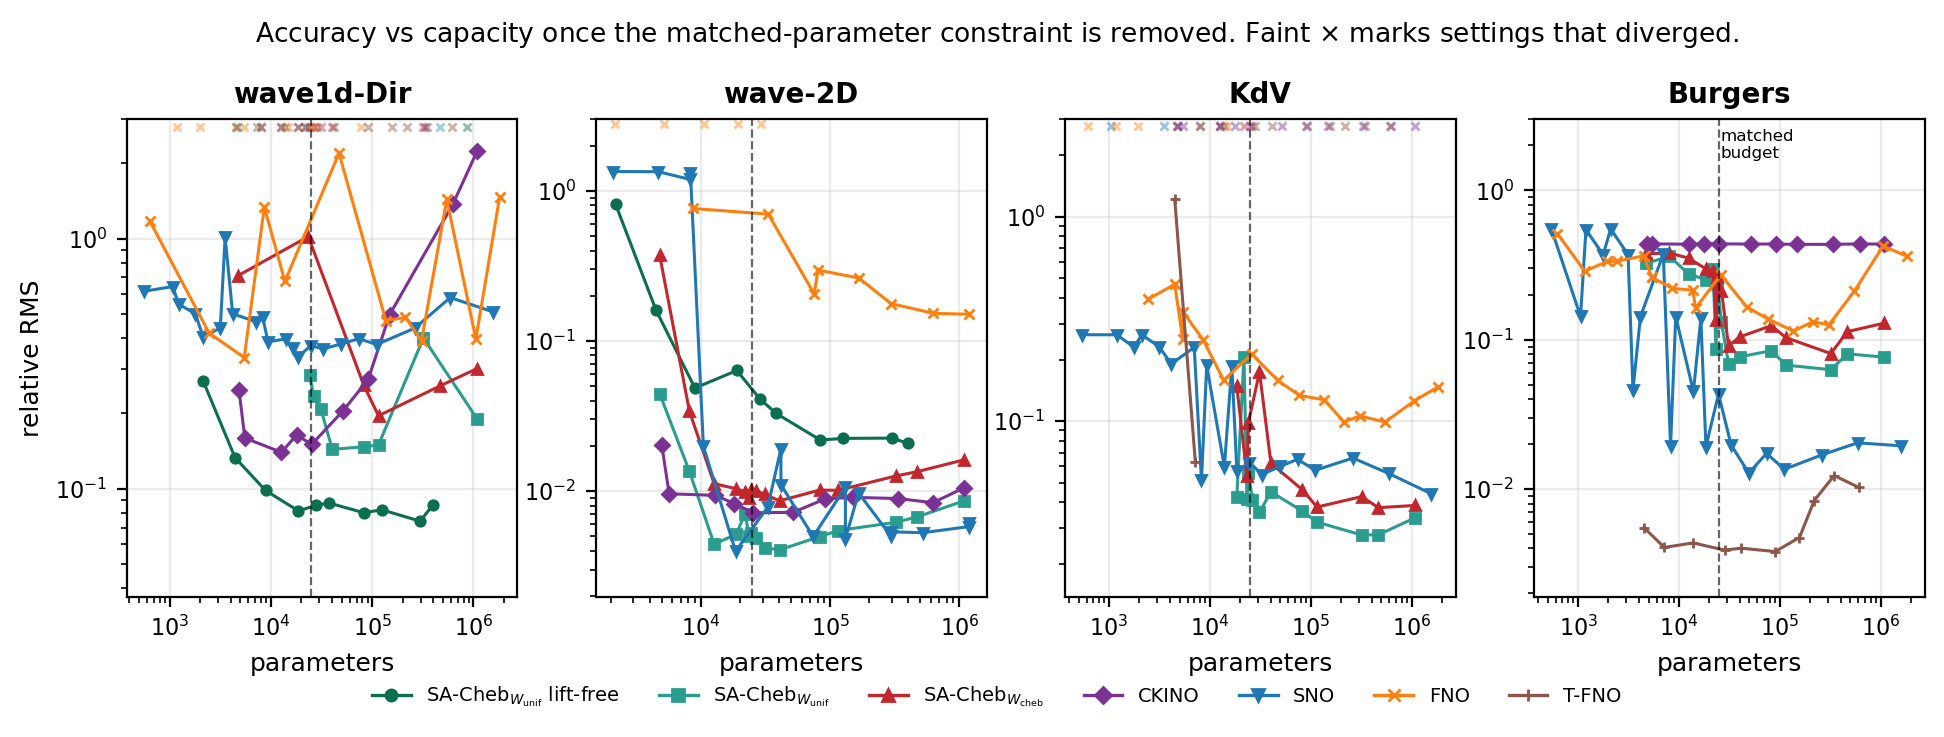
\includegraphics[width=\linewidth]{figs/capacity.png}
\caption{Accuracy against parameter count with the matched budget removed; the
dashed line marks the 25k budget used in Table~\ref{tab:winners}. The ranking is
budget-dependent, so the matched table should be read as ``best at 25k'' rather
than ``best architecture''.}
\label{fig:capacity}
\end{figure}

Two observations. On \texttt{wave1d\_dir} the two end-to-end symplectic models
take the top two slots outright ($0.0742$ and $0.0755$), the only problem where
they win the unconstrained comparison, and the only Hamiltonian non-periodic one.
And cost-efficiency diverges sharply from peak accuracy: on \texttt{wave3d} SNO's
$0.00271$ costs $1.36$M parameters while \texttt{sacheb\_naive} reaches $0.00345$
with $49{,}750$, \textbf{27$\times$ cheaper for $1.3\times$ worse}.

\subsection{Repeat execution: a standard we think this literature needs}
\label{sec:repro}

Operator-learning results are rarely re-run, including by their own authors.
Seed counts of three are common, margins of a few percent are reported as wins,
and there is usually no way for a reader to tell which of those wins would
survive re-running the study. We are in a position to check, because the entire
matrix, all $783$ runs, was executed twice on the cluster. The duplication was
not planned, but treating it as a control is the most useful thing we can do with
it, and we argue the practice should be routine rather than accidental.

We call this a repeat execution rather than a replication, and the distinction is
worth keeping. Both executions share an implementation, an experimental design, a
cluster and a set of authors; what differs between them is only what a re-run
varies, namely scheduling, hardware assignment and kernel-level nondeterminism.
It therefore bounds how much of the study is an artefact of one particular
execution. It says nothing about whether an independent group writing an
independent implementation would reach the same conclusions, which is what
replication properly means and is not something authors can certify for
themselves.

\begin{table}[htbp]
\centering
\caption{Every headline claim under a full re-execution of the study.}
\label{tab:repro}
\small
\begin{tabular}{@{}lccl@{}}
\toprule
claim & execution A & execution B & verdict \\
\midrule
form ablation (lifted) & $\Wu$ 16 / $\Wc$ 1 & $\Wu$ 16 / $\Wc$ 2 & \textbf{robust} \\
lift-free ratios & $17.2/1.24/21.6/14.2$ & identical & \textbf{robust} \\
long-horizon boundedness & lift-free only & lift-free only & \textbf{robust} \\
winner, 8 of 9 problems & & & \textbf{stable} \\
winner, advection & \ckino{} $0.001092$ & SNO $0.001196$ & \emph{flipped} \\
\bottomrule
\end{tabular}
\end{table}

The one claim that did not survive is instructive. On advection the contending
Chebyshev configuration varies by $15.7\times$ across seeds ($0.00062$ to
$0.00968$) against SNO's $1.4\times$. That is not a close race between two good
models; it is one unstable configuration occasionally landing well. Under a
single execution it would have been reported as a win for our own operator. We
report advection as a tie.

Two things follow. First, as a methodological rule: \textbf{with three seeds, a
difference smaller than the seed spread is not a result}. Every claim we advance
in \S\ref{sec:intro-claims} survived re-execution with margins of
$1.4$--$22\times$; the single claim that did not had a margin of $1.1\times$.
Second, as a reporting standard: the seed spread should be published alongside
the mean, because it is what tells a reader whether a margin is load-bearing.
We report both throughout.

\subsection{Supporting axes}
\label{sec:support}

\paragraph{Darcy (elliptic, Dirichlet).} \ckino{} attains $8.7\times$ lower
relative $L^2$ error than FNO overall and $18.3\times$ lower \emph{at the
boundary}, transferring zero-shot from $64^2$ to $128^2$. This is the clearest
non-periodic win for the Chebyshev basis.

\paragraph{Capacity ceilings.} A 6k--400k sweep shows \ckino{}'s Burgers failure
is \emph{representational}, flat at $\approx0.25$ across a $60\times$ range, and
its recursive KdV instability persists at every budget. Neither is fixed by scale.

\paragraph{Discretisation invariance.} Training at $N=64$ and evaluating at
$N=128$, \textbf{SNO and T-FNO win this axis outright}: they are essentially
exactly invariant ($0.99$--$1.00$) \emph{and} accurate, which is the combination
that matters. \ckino{} with a convolutional lift degrades by $57\times$ on
advection; the spectral lift restores invariance ($0.998$) but costs two to three
orders of magnitude of accuracy at the training grid
($8.2\times10^{-4}\!\to\!0.475$). There is no setting of our construction that is
both invariant and accurate, and we do not have a fix. If a workflow requires
evaluating at a resolution it did not train on, that is a decisive argument for
the Fourier family and against ours.

\paragraph{Inference speed.} Operators beat the reference solver only where the
solver is expensive: FNO is $3.2\times$ on Burgers, $7.7\times$ on KdV and
$5.8\times$ on \texttt{ns2d}; \ckino{} is $2.3\times$ on KdV but $0.07\times$ on
advection.

% ============================================================================
\section{Where each construction wins}
\label{sec:verdict}
% ============================================================================

\begin{table}[htbp]
\centering
\caption{Honest summary. No single operator dominates; the axes separate, and
two of the four axes go to the Fourier family.}
\label{tab:verdict}
\small
\begin{tabular}{@{}lp{56mm}p{48mm}@{}}
\toprule
construction & wins & loses \\
\midrule
\texttt{pureunif} (lift-free, $\Wu$)
 & long horizon (only bounded operator at $2\times10^{4}$ steps); \texttt{wave3d} at 25k; top of the unconstrained \texttt{wave1d\_dir} sweep
 & needs a canonical $(q,p)$ pair, so undefined on scalar fields; limited capacity per parameter \\
\addlinespace
\texttt{sacheb\_naive} (lifted, $\Wu$)
 & \texttt{wave1d\_dir}, \texttt{wave2d}, \texttt{ns2d} at 25k; best accuracy-per-parameter in $3$-D
 & no long-horizon guarantee; diverges like the rest at $10^4$ steps \\
\addlinespace
\ckino{}
 & advection/heat unconstrained by $10^{2}$--$10^{3}\times$; Darcy by $8.7\times$ ($18.3\times$ at the boundary)
 & not symplectic in any form; Burgers ceiling; KdV instability; worst discretisation invariance in the study \\
\addlinespace
SNO \citep{makara2026sno}
 & KdV outright, and ties advection, \texttt{wave1d} and \texttt{wave2d}; \textbf{discretisation invariance outright}; competitive in $2$-D
 & Fourier basis mismatched on non-periodic domains ($6.5\times$ on \texttt{wave1d\_dir}); expensive in $3$-D ($1.36$M parameters for its best) \\
\addlinespace
T-FNO \citep{kossaifi2023mgtfno}
 & heat, Burgers; invariance
 & no structure; long-horizon divergence \\
\bottomrule
\end{tabular}
\end{table}

We want to be explicit about the shape of this table rather than let it be read
selectively. Counting a problem as a tie whenever the gap between the two best
families is smaller than the sum of their seed standard deviations, the rule \S\ref{sec:repro} argues for, only \emph{five} of the nine problems have a clear
winner: \texttt{wave1d\_dir}, \texttt{wave3d} and \texttt{ns2d} to our
construction, KdV to SNO, Burgers to T-FNO. The remaining four (advection, heat,
\texttt{wave1d}, \texttt{wave2d}) are ties. Splitting ties evenly the tally is
ours $5.0$, SNO $2.5$, T-FNO $1.5$.

Our construction wins the two axes it was designed for: behaviour under long rollout, and accuracy on non-periodic and multi-dimensional domains. It loses the
two it was not. \textbf{SNO wins discretisation invariance outright}, being
simultaneously invariant and accurate where our operator can be only one or the
other, and the Fourier family wins or ties every periodic $1$-D problem. A reader
whose workload is periodic, or who must evaluate at a resolution the model was
not trained on, should use a Fourier operator.

% ============================================================================
\section{Limitations}
\label{sec:limits}
% ============================================================================

\textbf{The matching hypothesis is tested in one direction only.} This is the
most important gap in the study. Every benchmark here is sampled on a uniform
grid, so $\Wu$ is the matched form in all nine experiments and $\Wc$ is the
mismatched one in all nine (Table~\ref{tab:nodes}). The ablation therefore
establishes that the mismatched form loses; it does not on its own separate that
explanation from the simpler one that constant weights are just the better
choice. The decisive control is a dataset genuinely discretised on CGL nodes,
where $\Wc$ becomes the physically correct quadrature and the preference should
\emph{reverse}. We have not run it. Until it is run, the claim that the inner
product must match the discretisation should be read as strongly suggested by
Theorem~\ref{thm:sacheb} and Proposition~\ref{prop:necessity}, and consistent
with the measurements, rather than as established by them.

\textbf{Winner selection in Table~\ref{tab:winners}.} The best configuration per
problem is chosen on the test split rather than on validation, so those
per-problem numbers are optimistic by an unquantified amount
(\S\ref{sec:splits}). The paired comparisons the argument rests on are not
affected, since they are pre-specified rather than selected.

\textbf{The wrapper is removed as a unit.} \S\ref{sec:long} contrasts a lifted
operator with a lift-free one, but that single change removes the lift, the
projection and the residual update at once, and additionally forces $H=C$. The
experiments therefore identify the conventional wrapper as a whole as the thing
that forfeits the guarantee; they do not apportion blame among its three parts. A
staged ablation that restores each component separately, and a variant whose lift
and projection are themselves canonical transformations, would settle which one
matters.

\textbf{Parameter count is the only matched resource.} Equal parameters does not
mean equal FLOPs, memory or wall-clock across families with arithmetic profiles
as different as these (\S\ref{sec:design}); accuracy comparisons here should not
be read as efficiency comparisons.

\textbf{Re-implementations.} SNO and GENERIC-FNO are our implementations from the
published descriptions and were not tuned to the authors' protocols.

\textbf{Our GENERIC-FNO bug.} It diverged in all 12 entries. Parameterising the
PSD multiplier as $M=b^2$ with $b$ initialised at zero places it at a saddle
($\partial M/\partial b=2b=0$), so the dissipative channel never activates. This
is a defect of our implementation, \emph{not} evidence about the published
method, and no conclusion should be drawn from those rows.

\textbf{Canonical structure only.} The lift-free construction needs a canonical
$(q,p)$ pair and is therefore undefined on the scalar-field problems (advection,
heat, Burgers, KdV, \texttt{ns2d}). KdV is Hamiltonian only under the
non-canonical Gardner bracket, which we do not cover.

\textbf{Scale and horizon.} Domains are small ($32$--$64$ points in $1$-D, $32^2$,
$16^3$, $64^2$), adequate to resolve the reported orderings but not a deployment
benchmark. $2\times10^{4}$ steps separates bounded from unbounded but is still far
short of the regimes where backward-error analysis is usually invoked.

\textbf{Single hardware.} All $783$ runs used one accelerator type (Tesla T4)
with TF32 disabled, so arithmetic is consistent across the matrix; results may
differ on accelerators with different defaults.

% ============================================================================
\section{Conclusion}
% ============================================================================

We set out to test whether geometric structure helps a learned operator and found
that the question, as usually posed, is incomplete. Symplecticity is defined
relative to an inner product; on a non-uniform grid two reasonable
implementations preserve two different forms, both exactly, and only measurement
distinguishes them. Once the form is named the picture is clean: on the uniform
grids these benchmarks use, the form matching the discretisation wins $16$ of
$18$ comparisons, and $4$ of $4$ by an order of magnitude more when the deployed
map, rather than merely its core, carries the guarantee. That same construction
is the only one in our study to survive a $2\times10^{4}$-step rollout, and it
survives bounded rather than accurate. Structure preservation pays; it is simply
forfeited by the wrapper the field conventionally puts around it, and invisible
unless you say with respect to what. We also retract a symplecticity theorem of
our own that mistook unit Jacobian determinant for preservation of $\omega$, and
we think the general lesson is that such claims should be measured rather than
argued: the measurement needs only standard JVP and VJP calls and never forms
the Jacobian.

% ============================================================================
\begin{thebibliography}{99}\small
% ============================================================================

\bibitem[Cranmer et al.(2020)]{cranmer2020lnn}
M.~Cranmer, S.~Greydanus, S.~Hoyer, P.~Battaglia, D.~Spergel, and S.~Ho.
\newblock Lagrangian Neural Networks.
\newblock \emph{ICLR 2020 Workshop on Integration of Deep Neural Models and
Differential Equations}, 2020. arXiv:2003.04630.

\bibitem[Duruisseaux et al.(2026)]{duruisseaux2026fnoexplained}
V.~Duruisseaux, J.~Kossaifi, and A.~Anandkumar.
\newblock Fourier Neural Operators Explained: A Practical Perspective.
\newblock arXiv:2512.01421, 2026.

\bibitem[Finzi et al.(2020)]{finzi2020lieconv}
M.~Finzi, S.~Stanton, P.~Izmailov, and A.~G. Wilson.
\newblock Generalizing Convolutional Neural Networks for Equivariance to Lie
Groups on Arbitrary Continuous Data.
\newblock \emph{ICML}, 2020. arXiv:2002.12880.

\bibitem[Greydanus et al.(2019)]{greydanus2019hnn}
S.~Greydanus, M.~Dzamba, and J.~Yosinski.
\newblock Hamiltonian Neural Networks.
\newblock \emph{NeurIPS}, 2019. arXiv:1906.01563.

\bibitem[Grmela and \"Ottinger(1997)]{grmela1997generic}
M.~Grmela and H.~C. \"Ottinger.
\newblock Dynamics and thermodynamics of complex fluids. I. Development of a
general formalism.
\newblock \emph{Physical Review E}, 56(6):6620--6632, 1997.

\bibitem[Hairer et al.(2006)]{hairer2006gni}
E.~Hairer, C.~Lubich, and G.~Wanner.
\newblock \emph{Geometric Numerical Integration: Structure-Preserving Algorithms
for Ordinary Differential Equations}.
\newblock Springer Series in Computational Mathematics, Vol.~31, 2nd edition,
Springer, 2006.

\bibitem[Jin et al.(2020)]{jin2020sympnets}
P.~Jin, Z.~Zhang, A.~Zhu, Y.~Tang, and G.~E. Karniadakis.
\newblock SympNets: Intrinsic structure-preserving symplectic networks for
identifying Hamiltonian systems.
\newblock \emph{Neural Networks}, 132:166--179, 2020. arXiv:2001.03750.

\bibitem[Kossaifi et al.(2023)]{kossaifi2023mgtfno}
J.~Kossaifi, N.~Kovachki, K.~Azizzadenesheli, and A.~Anandkumar.
\newblock Multi-Grid Tensorized Fourier Neural Operator for High-Resolution
PDEs.
\newblock arXiv:2310.00120, 2023.

\bibitem[Kossaifi et al.(2024)]{kossaifi2024library}
J.~Kossaifi, N.~Kovachki, Z.~Li, D.~Pitt, M.~Liu-Schiaffini, R.~J. George,
B.~Bonev, K.~Azizzadenesheli, J.~Berner, V.~Duruisseaux, and A.~Anandkumar.
\newblock A Library for Learning Neural Operators.
\newblock arXiv:2412.10354, 2024.

\bibitem[Kovachki et al.(2023)]{kovachki2023neural}
N.~Kovachki, Z.~Li, B.~Liu, K.~Azizzadenesheli, K.~Bhattacharya, A.~Stuart, and
A.~Anandkumar.
\newblock Neural Operator: Learning Maps Between Function Spaces with
Applications to PDEs.
\newblock \emph{Journal of Machine Learning Research}, 24(89):4061--4157, 2023.
arXiv:2108.08481.

\bibitem[Li et al.(2021)]{li2021fno}
Z.~Li, N.~Kovachki, K.~Azizzadenesheli, B.~Liu, K.~Bhattacharya, A.~Stuart, and
A.~Anandkumar.
\newblock Fourier Neural Operator for Parametric Partial Differential Equations.
\newblock \emph{ICLR}, 2021. arXiv:2010.08895.

\bibitem[Li et al.(2023)]{li2023pino}
Z.~Li, H.~Zheng, N.~Kovachki, D.~Jin, H.~Chen, B.~Liu, K.~Azizzadenesheli, and
A.~Anandkumar.
\newblock Physics-Informed Neural Operator for Learning Partial Differential
Equations.
\newblock arXiv:2111.03794, 2023.

\bibitem[Lu et al.(2021)]{lu2021deeponet}
L.~Lu, P.~Jin, and G.~E. Karniadakis.
\newblock Learning nonlinear operators via DeepONet based on the universal
approximation theorem of operators.
\newblock \emph{Nature Machine Intelligence}, 3(3):218--229, 2021.
arXiv:1910.03193.

\bibitem[Makara et al.(2026)]{makara2026sno}
Y.~Makara, Y.~Tanaka, T.~Matsubara, and T.~Yaguchi.
\newblock Symplectic Neural Operators for Learning Infinite Dimensional
Hamiltonian Systems.
\newblock arXiv:2605.15881, 2026.

\bibitem[Marsden and Ratiu(1999)]{marsden1999mechanics}
J.~E. Marsden and T.~S. Ratiu.
\newblock \emph{Introduction to Mechanics and Symmetry: A Basic Exposition of
Classical Mechanical Systems}.
\newblock Texts in Applied Mathematics, Vol.~17, 2nd edition, Springer, 1999.

\bibitem[\"Ottinger(2005)]{ottinger2005beyond}
H.~C. \"Ottinger.
\newblock \emph{Beyond Equilibrium Thermodynamics}.
\newblock Wiley-Interscience, Hoboken, NJ, 2005.

\bibitem[Perez et al.(2018)]{perez2018film}
E.~Perez, F.~Strub, H.~de~Vries, V.~Dumoulin, and A.~Courville.
\newblock FiLM: Visual Reasoning with a General Conditioning Layer.
\newblock \emph{AAAI}, 2018. arXiv:1709.07871.

\bibitem[Raissi et al.(2019)]{raissi2019pinn}
M.~Raissi, P.~Perdikaris, and G.~E. Karniadakis.
\newblock Physics-informed neural networks: A deep learning framework for
solving forward and inverse problems involving nonlinear partial differential
equations.
\newblock \emph{Journal of Computational Physics}, 378:686--707, 2019.

\bibitem[Sulskis and Ravi(2026)]{sulskis2026generic}
J.~Sulskis and S.~Ravi.
\newblock GENERIC-FNO: Embedding Energy Conservation and Entropy Production into
Fourier Neural Operators.
\newblock arXiv:2606.08343, 2026.

\bibitem[Trefethen(2000)]{trefethen2000spectral}
L.~N. Trefethen.
\newblock \emph{Spectral Methods in MATLAB}.
\newblock SIAM, Philadelphia, 2000.

\bibitem[Varghese et al.(2026)]{varghese2026pisonet}
A.~J. Varghese, S.~Liu, P.~Chen, Y.~Zhu, J.~Darbon, and G.~E. Karniadakis.
\newblock PI-SONet: A Physics-Informed Symplectic Operator Network for
Real-Time Optimal Control of Multi-Agent Systems.
\newblock arXiv:2605.14332, 2026.

\bibitem[Weinstein(1969)]{weinstein1969symplectic}
A.~Weinstein.
\newblock Symplectic structures on Banach manifolds.
\newblock \emph{Bulletin of the American Mathematical Society}, 75:1040--1041,
1969.

\bibitem[Wen et al.(2022)]{wen2022ufno}
G.~Wen, Z.~Li, K.~Azizzadenesheli, A.~Anandkumar, and S.~M. Benson.
\newblock U-FNO---An enhanced Fourier neural operator-based deep-learning model
for multiphase flow.
\newblock \emph{Advances in Water Resources}, 163:104180, 2022.
arXiv:2109.03697.

\bibitem[Zhang et al.(2022)]{zhang2022gfinns}
Z.~Zhang, Y.~Shin, and G.~E. Karniadakis.
\newblock GFINNs: GENERIC formalism informed neural networks for deterministic
and stochastic dynamical systems.
\newblock \emph{Philosophical Transactions of the Royal Society A},
380(2229):20210207, 2022.

\bibitem[Zhang et al.(2026)]{zhang2026legonet}
J.~Zhang, Y.~Wang, and G.~Lin.
\newblock LegONet: Plug-and-Play Structure-Preserving Neural Operator Blocks for
Compositional PDE Learning.
\newblock arXiv:2603.07882, 2026.

\bibitem[Zhong et al.(2020)]{zhong2020symoden}
Y.~D. Zhong, B.~Dey, and A.~Chakraborty.
\newblock Symplectic ODE-Net: Learning Hamiltonian Dynamics with Control.
\newblock \emph{ICLR}, 2020. arXiv:1909.12077.

\end{thebibliography}

\appendix
% ============================================================================
\section{Retraction of a previously asserted guarantee}
\label{app:retraction}
% ============================================================================

The \ckino{} operator was originally documented with an exact symplecticity
theorem. We retract it, and record the error because it is instructive.

The withdrawn argument ran: each St\"ormer--Verlet substep has a Jacobian that is
triangular with unit diagonal blocks, hence determinant $1$, hence preserves
$\omega$. The step from ``determinant $1$'' to ``preserves $\omega$'' is invalid.
By Proposition~\ref{prop:shear}, $\det D\Phi=1$ holds for every shear, while
preservation of $\omega_W$ additionally requires $WA=A^{\top}W$. The operator's
kernel \eqref{eq:ckino-kernel} uses independent $\varphi_r,\psi_r$ and an
unconstrained channel mix, so $A$ is not self-adjoint; the measured defect is
$\approx1.4$ in \emph{both} candidate forms (Figure~\ref{fig:defect}). A corollary
energy-drift bound, whose proof invoked the modified-Hamiltonian machinery of
backward error analysis \citep{hairer2006gni}, is retracted with it: that
machinery requires symplecticity, and volume preservation alone does not imply
the existence of a modified Hamiltonian.

A second, subtler retraction concerns the comparison itself. An earlier draft
reported that exact symplecticity was a measurable cost, on the basis of a
defect table computed against a single inner product. Scoring both variants
against both forms (Figure~\ref{fig:defect}) shows the ``non-symplectic'' control
was exactly symplectic in the uniform form all along, and reverses the
conclusion.

% ============================================================================
\section{The weighted adjoint in the low-rank basis}
\label{app:lowrank}
% ============================================================================

With $\alpha_r=\iprod{\psi_r}{v}_W$ and $(Kv)(x)=\sum_r\varphi_r(x)M_r\alpha_r$,
\[
\iprod{Kv}{g}_W
=\sum_r (M_r\alpha_r)^{\top}\iprod{\varphi_r}{g}_W
=\sum_r \alpha_r^{\top}\big(M_r^{\top}\iprod{\varphi_r}{g}_W\big)
=\Big\langle v,\;\sum_r \psi_r\,M_r^{\top}\iprod{\varphi_r}{g}_W\Big\rangle_W,
\]
which is exactly $\iprod{v}{K^{*}g}_W$. Hence the weighted adjoint is obtained by
exchanging $\varphi$ and $\psi$ and transposing the channel mixing; no inverse of
$W$ is formed and the cost remains $O(RN^d)$. In $d$ dimensions the weight is the
outer product of the per-axis weights and remains diagonal, so both this identity
and Theorem~\ref{thm:sacheb} carry over unchanged.

\end{document}
